\documentclass{beamer}
\usetheme{}
\usecolortheme{dolphin}           
\useinnertheme{circles}
\setbeamertemplate{itemize items}[default]
\setbeamertemplate{enumerate items}[default]
\usepackage[T1]{fontenc}
\usepackage[utf8]{inputenc}
\usepackage{lmodern}
\usepackage{amsmath}
\usepackage{booktabs} 
\usepackage{graphicx}        
\usepackage{array}
\usepackage{color}
\usepackage{textcomp}
\usepackage{epstopdf}                     % For EPS figures
\makeatletter
\def\zapcolorreset{\let\reset@color\relax\ignorespaces}
\def\colorrows#1{\noalign{\aftergroup\zapcolorreset#1}\ignorespaces}
\makeatother
%\graphicspath{{/home/swl/Dropbox/ucd/international_trade/tex/}} 
\setbeamertemplate{navigation symbols}{}

%--------------------------------------
%%%% DETAILS TITLE PAGE %%%%
%--------------------------------------
\title{International trade patterns}
\author{School of Economics, University College Dublin}
\date{Autumn 2017}
\begin{document}
%--------------------------------------
%%%% TITLE SLIDE %%%%
%--------------------------------------
\begin{frame}
\titlepage  
\end{frame}

%--------------------------------------
\begin{frame}{Port of Rotterdam (source: Daily Overview)}
  \begin{figure}\centering
    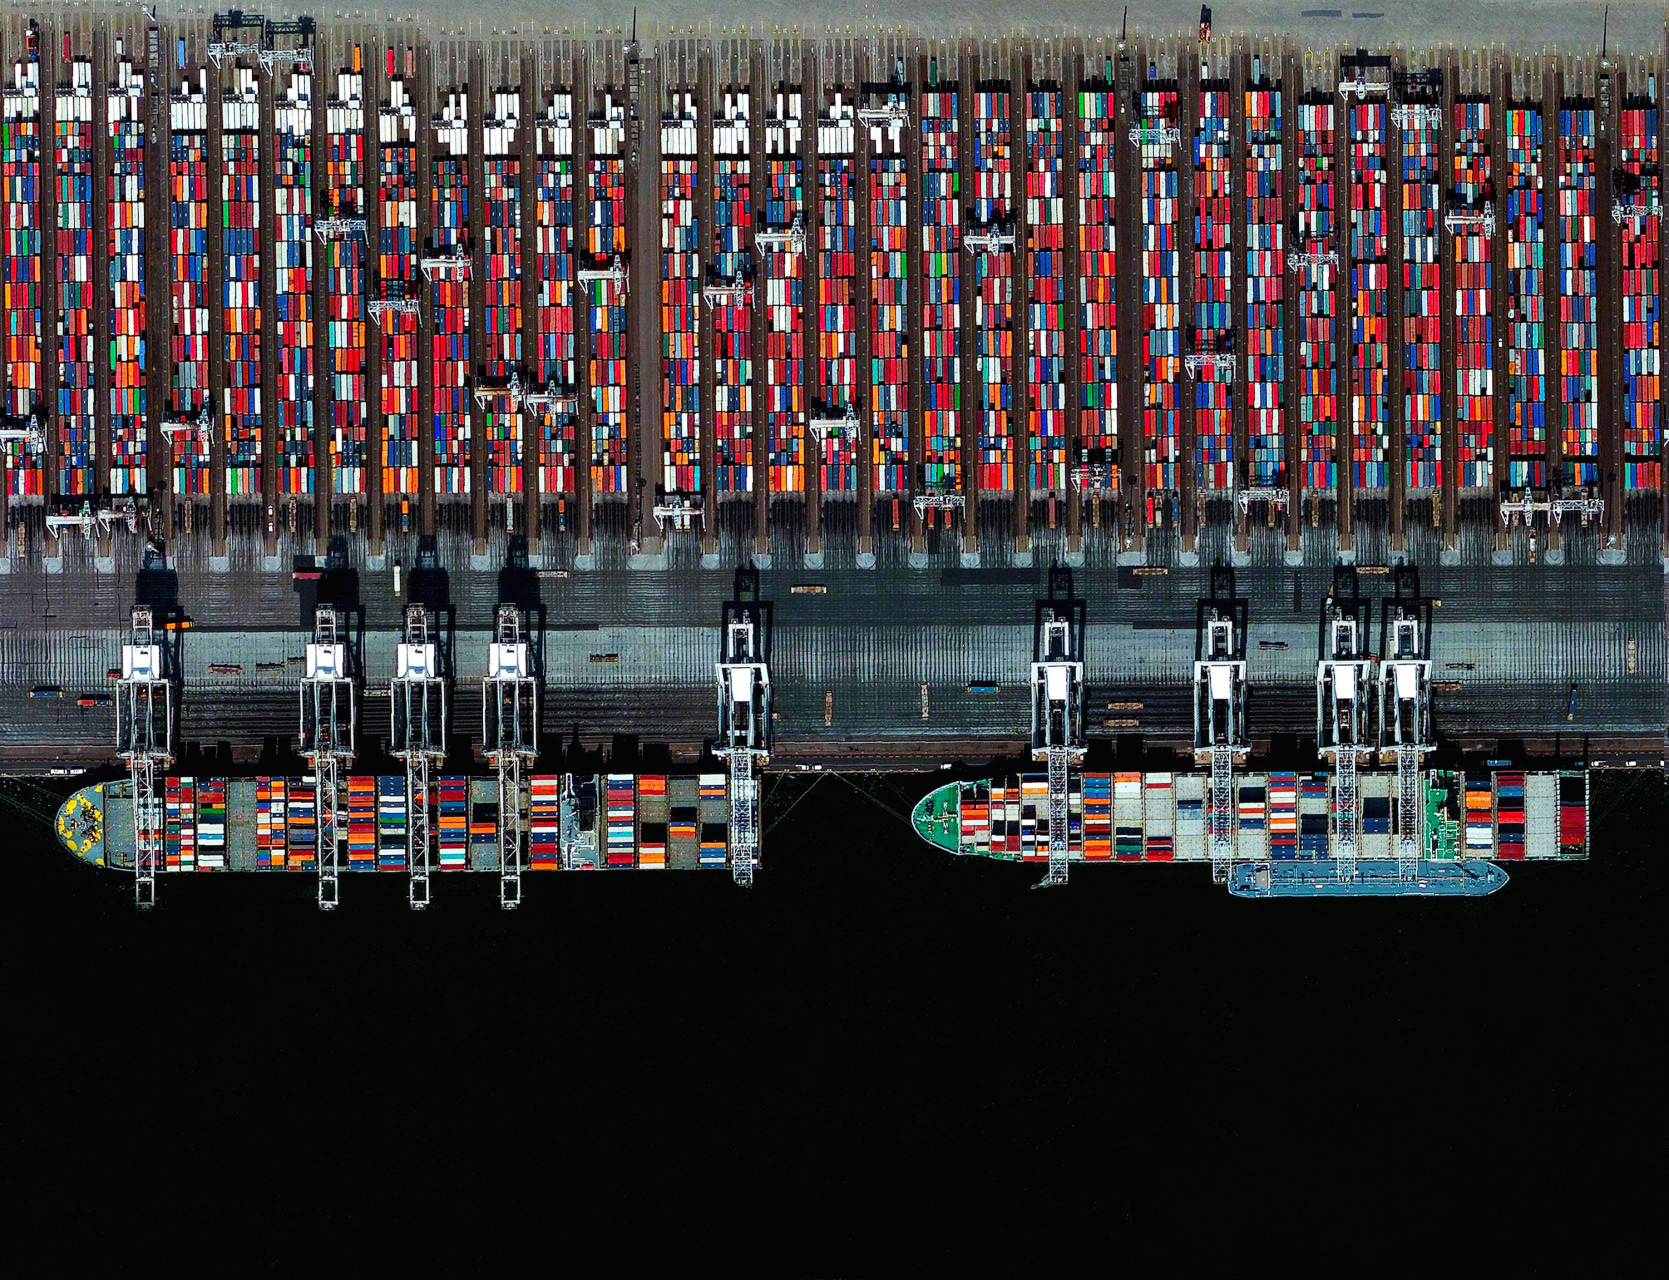
\includegraphics[scale=.17]{rotterdam}
  \end{figure}
\end{frame}
%--------------------------------------

%--------------------------------------
\begin{frame}
  Studying international trade we consider:\bigskip
  \begin{enumerate}
    \item Movement of goods and services from one country to another
    \begin{itemize}
      \item Merchandise goods: everything but services
      \item Services: transportation, insurance, etc. 
    \end{itemize}
    \medskip
    \item Movement of factors of production across countries
    \begin{itemize}
      \item Migration: flow of people/labour across borders
      \item Foreign Direct Investment: flow of capital across borders
    \end{itemize}
  \end{enumerate}
\end{frame}
%--------------------------------------

%--------------------------------------
\begin{frame}{}
  Countries trade goods and services with each other as it generates mutual benefits
  \begin{itemize}
    \item Norway imports oranges which they would have hard time producing
    \item Foreign produced goods could be cheaper or better in quality
  \end{itemize}
  \medskip
  Countries use finite resources to produce what they are most productive at and trade products for goods/services they want to consume
  \begin{itemize}
    \item Countries can specialise and still consume variety of goods/services through trade
  \end{itemize}

\end{frame}
%--------------------------------------

%--------------------------------------
\begin{frame}
  The main insight from most theories on international trade is that countries can gain through specialisation
  \begin{itemize}
    \item Export goods made with abundant resources, import goods made with relatively scarce resources
  \end{itemize}
  \medskip
  Specialisation leads to efficiency through large-scale production (economies of scale)
  \begin{itemize}
    \item Countries could benefit from international lending and migration as well
  \end{itemize}
\end{frame}
%--------------------------------------

%--------------------------------------
\begin{frame}
  Although in most theoretical models trade is predicted to benefit the whole country, particular groups might be harmed
  \begin{itemize}
    \item Owners of resources in industries that compete with imports
    \item Trade affects income distribution
  \end{itemize}
  \medskip
  Additionally, there are some who argue that trade might have a negative effect on the local environment.
\end{frame}
%--------------------------------------

%--------------------------------------
\begin{frame}{}
  We can track a country's imports $M$ and exports $X$ using the trade balance  
  \begin{align*}
    NX = X - M
  \end{align*}
  \begin{itemize}
    \item Trade surplus: $X>M$
    \item Trade deficit: $X<M$
  \end{itemize}
\end{frame}
%--------------------------------------

%--------------------------------------
\begin{frame}{Trade balance USA and China}
  \begin{figure}
    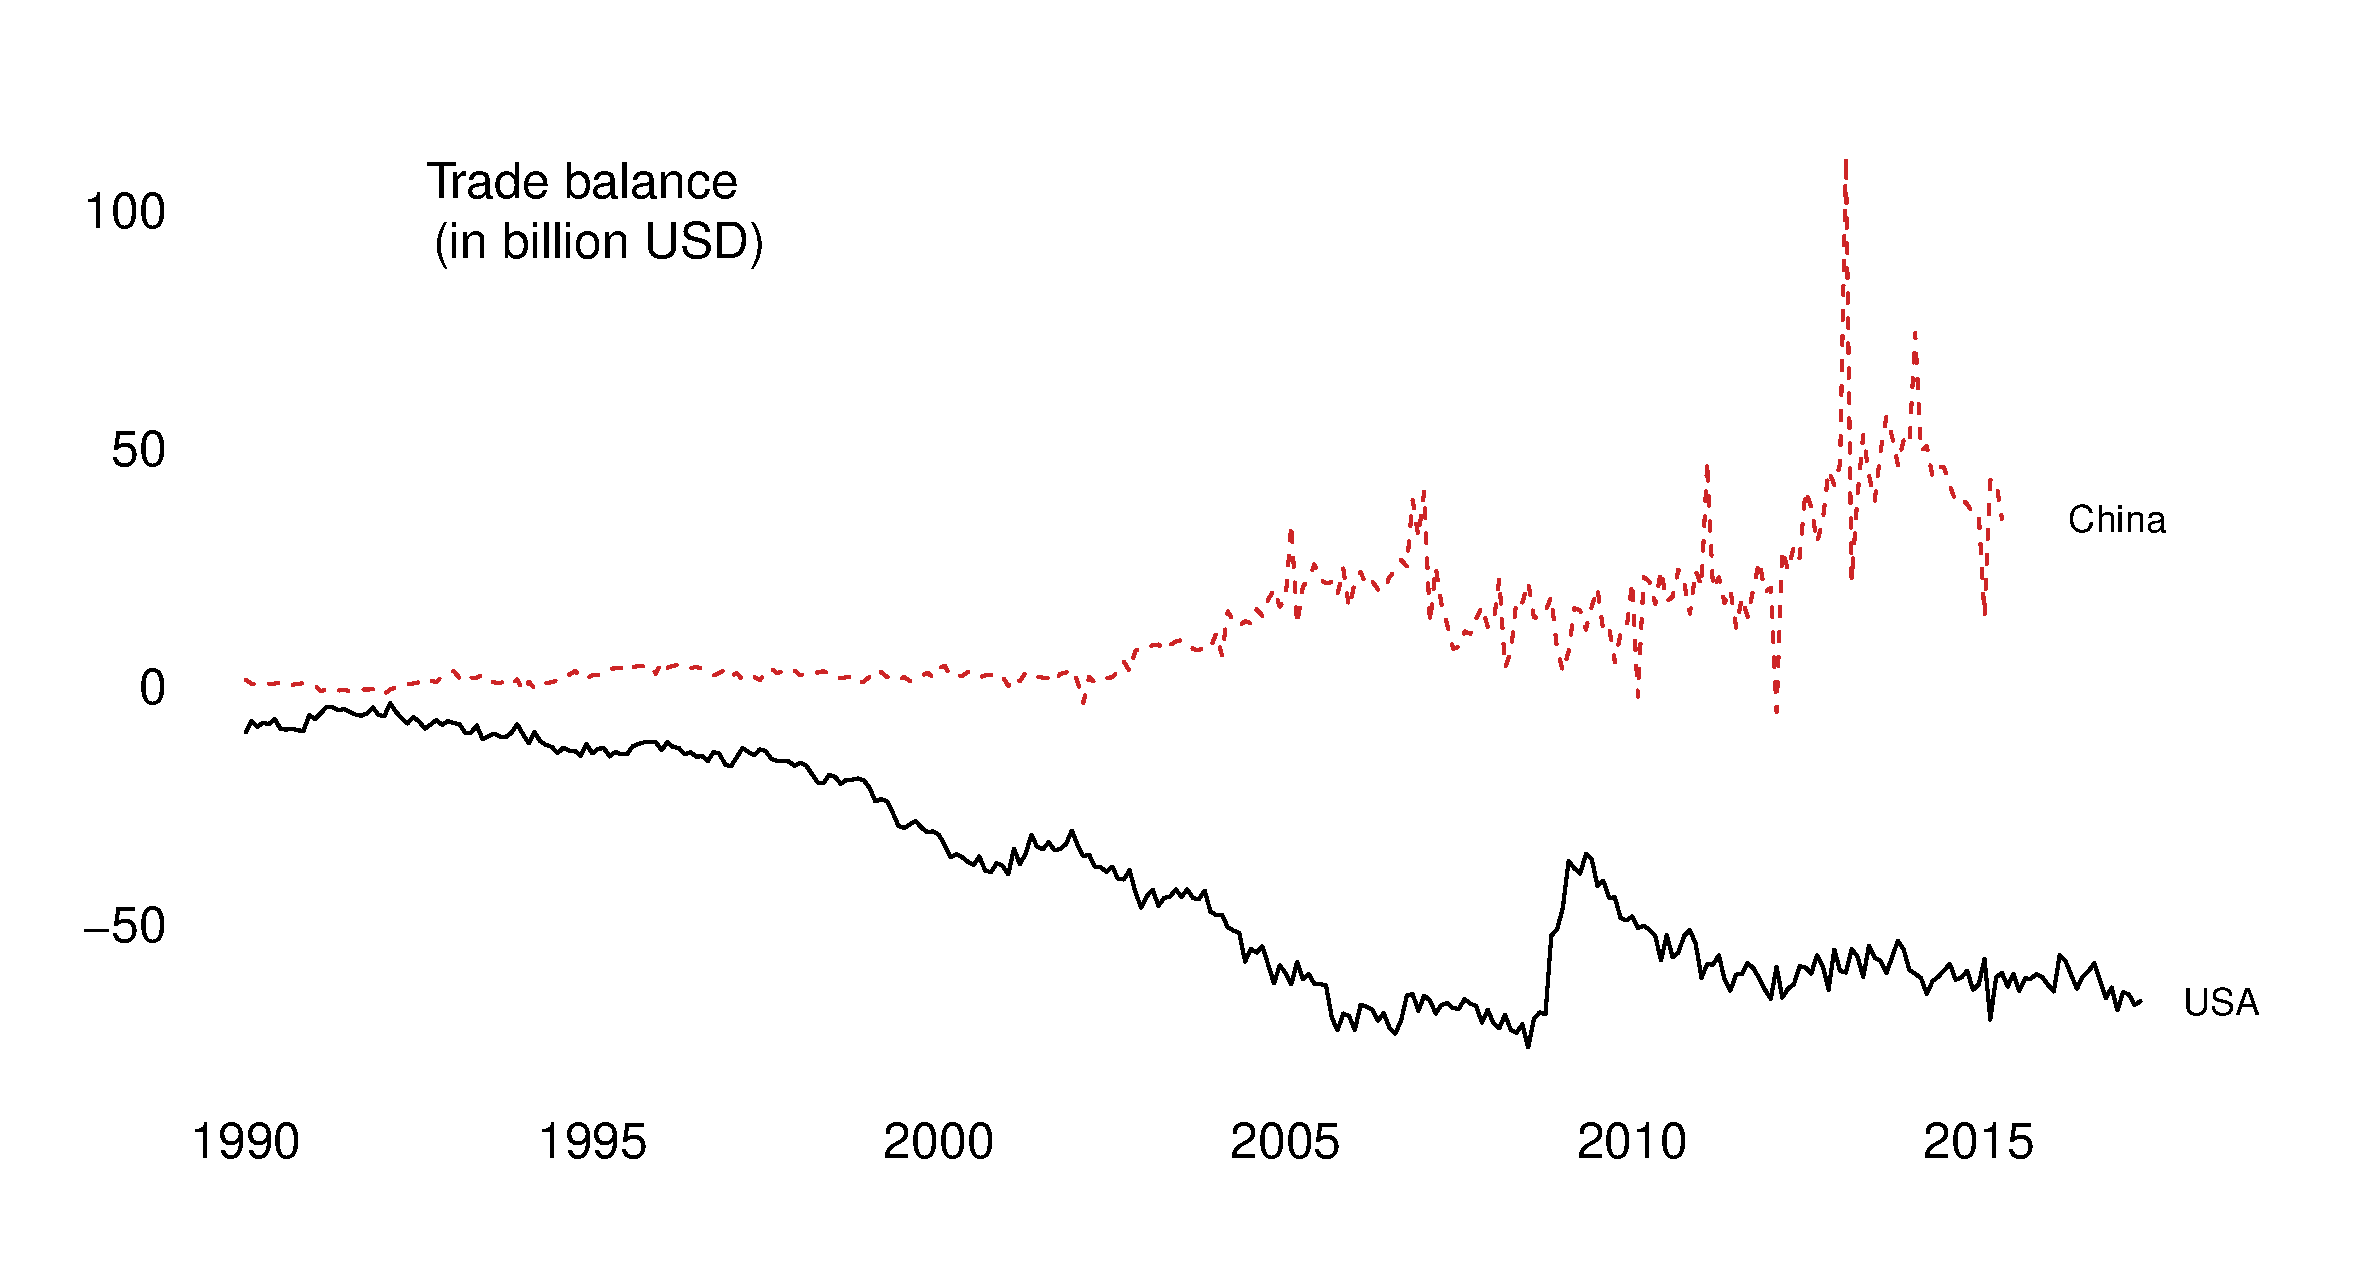
\includegraphics[scale=.3]{trade_balance}
  \end{figure}
  
\end{frame}
%--------------------------------------

%--------------------------------------
\begin{frame}{Bilateral trade balance USA and China}
  \begin{figure}
    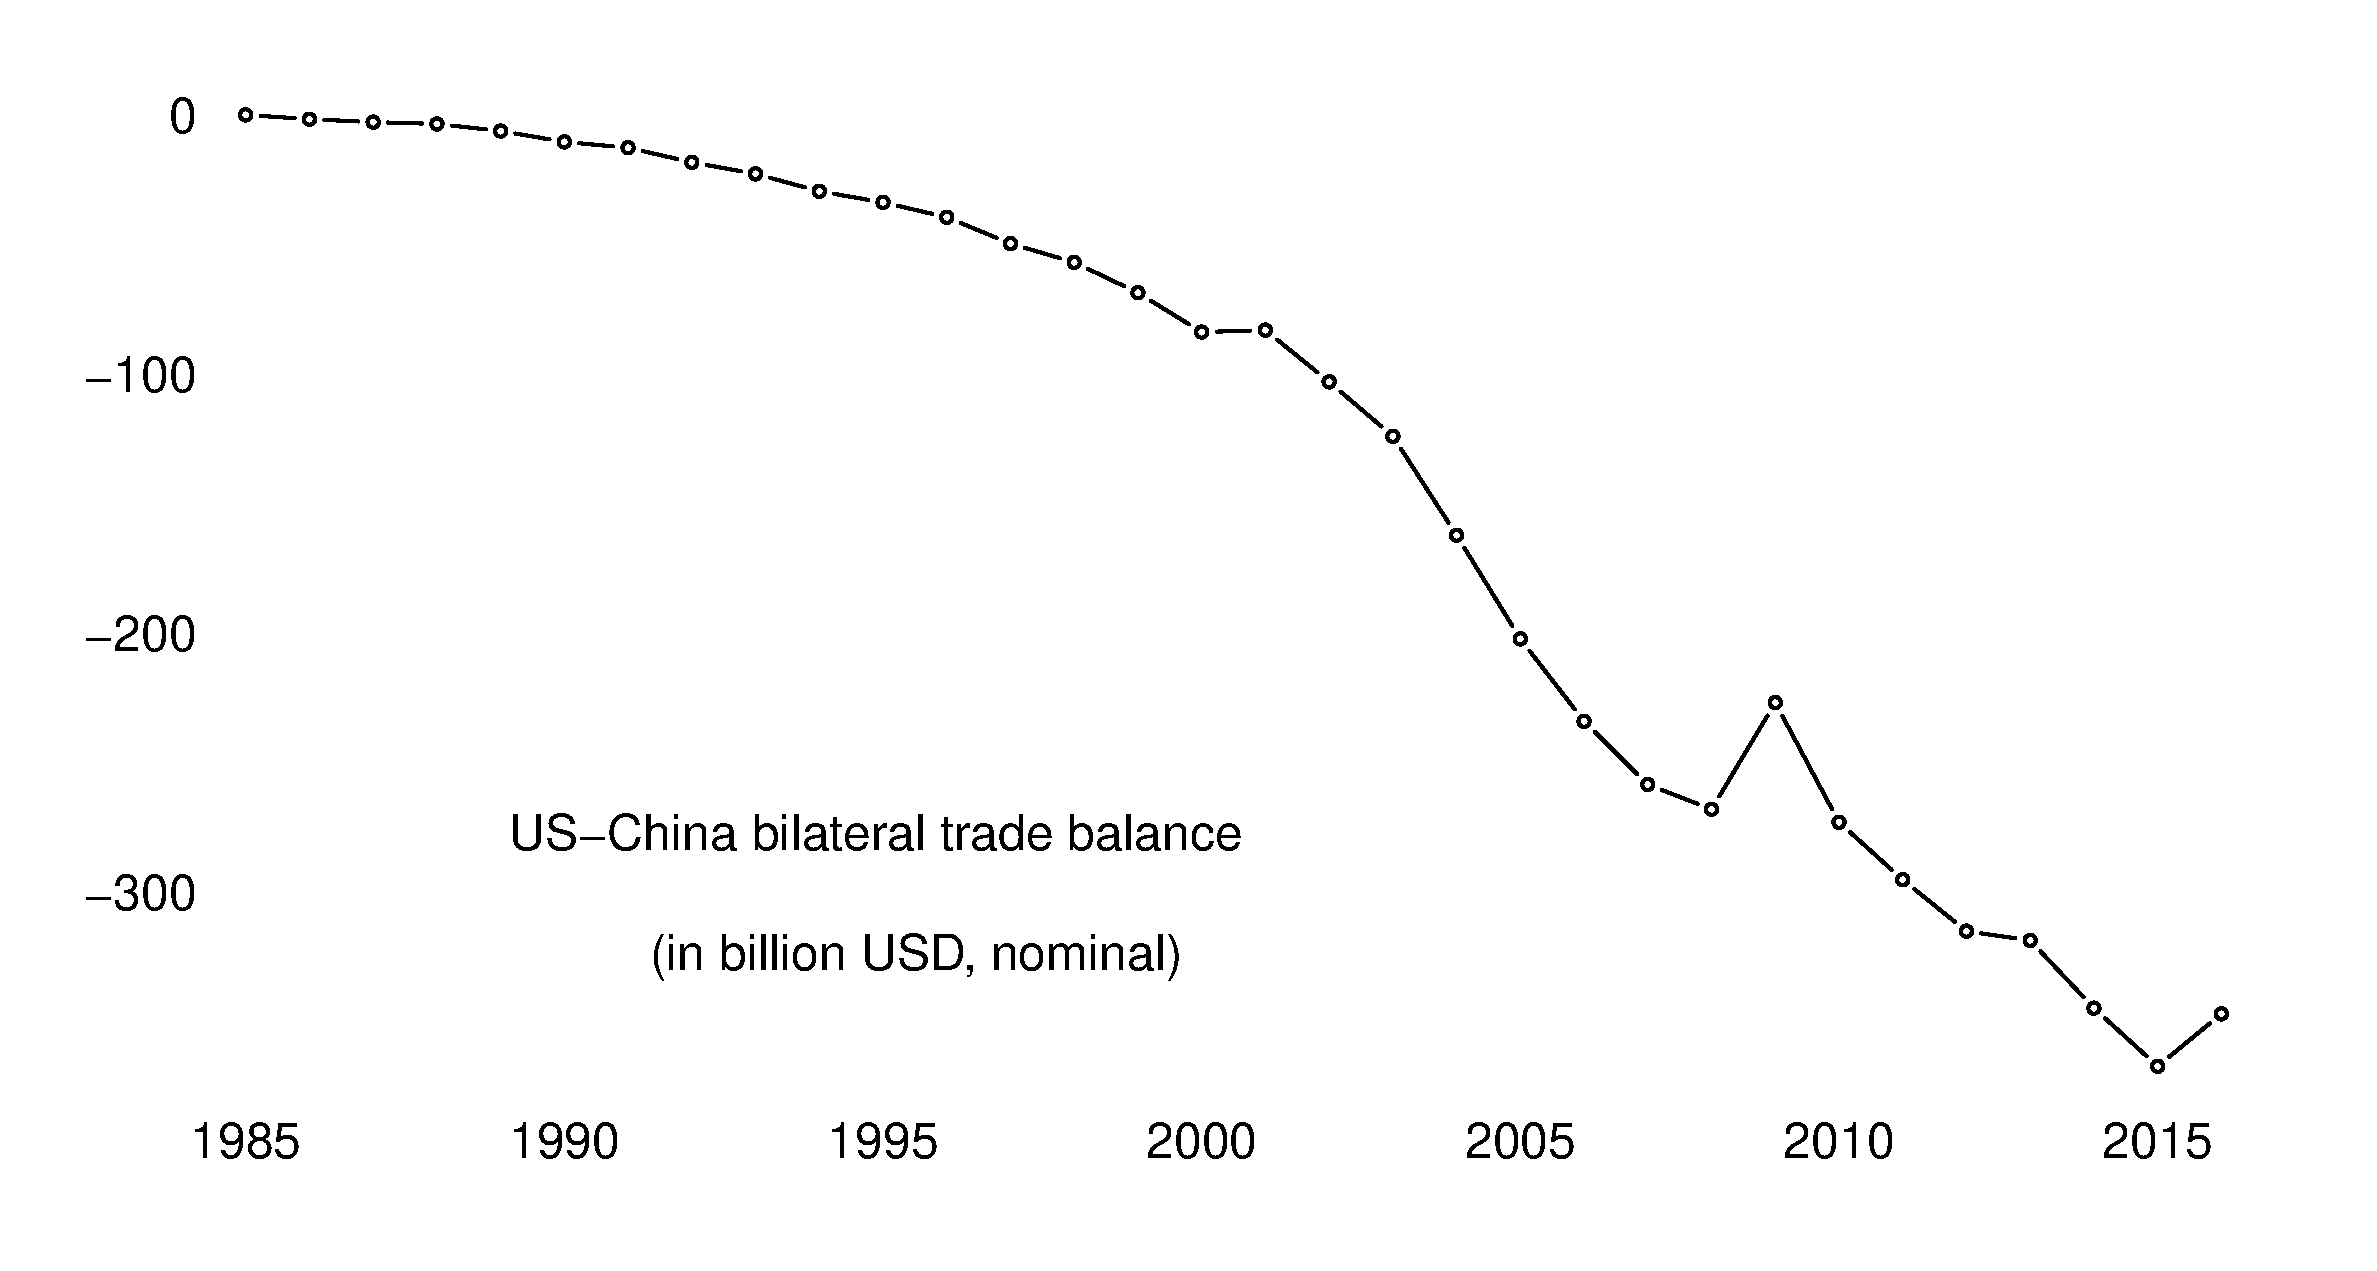
\includegraphics[scale=.3]{bilateral_balance}
  \end{figure}
\end{frame}
%--------------------------------------


%--------------------------------------
\begin{frame}{}
  \begin{figure}
    
\includegraphics[scale=.07]{lego}
  \end{figure}
  \begin{itemize}
    \item Valued at \texteuro 2 when imported to Ireland from Denmark
    \item Produced in Denmark but
    \begin{itemize}
      \item Plastic from Taiwan
      \item Paint produced in Czechia
      \item Packaging from Sweden
    \end{itemize}
    \item Value added in Denmark is $2-X$, with $X$ is total value of imported parts
  \end{itemize}
\end{frame}
%--------------------------------------

%--------------------------------------
\begin{frame}
  \begin{figure}\centering
    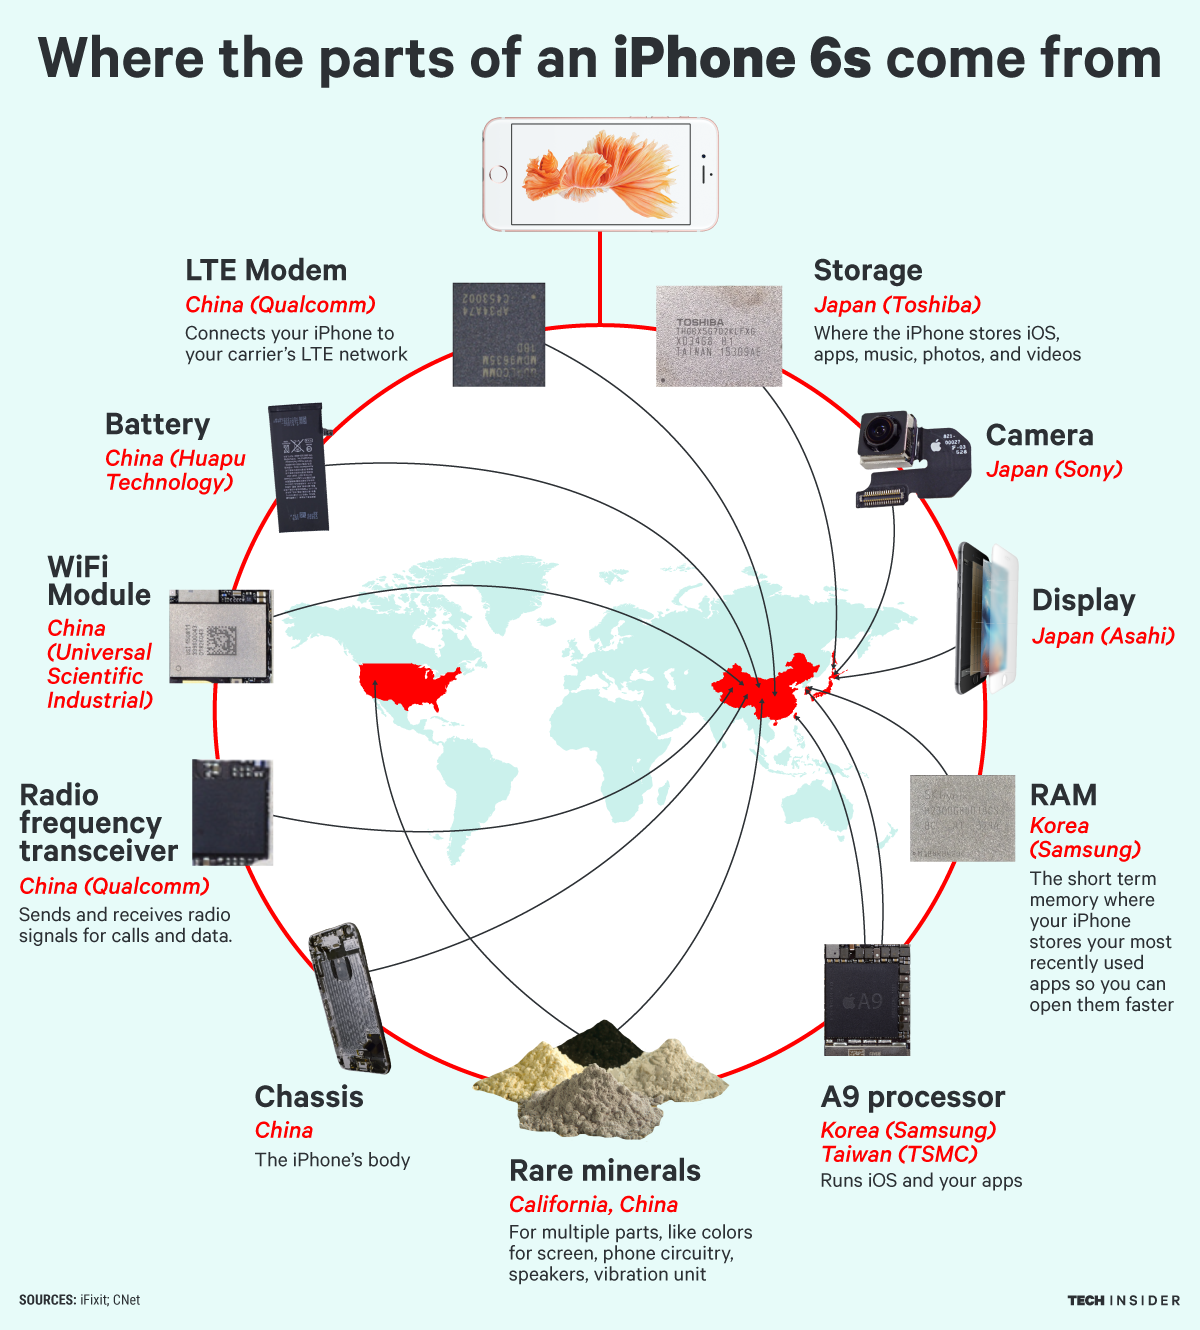
\includegraphics[scale=.2]{iphone6}
  \end{figure}
\end{frame}
%--------------------------------------

%--------------------------------------
\begin{frame}
  The trade balance has a shortcoming in measuring things such as bilateral trade because of the assumption that a country produces goods that are
  \begin{enumerate}
    \item Consumed domestically
    \item Exported
  \end{enumerate}
  Ignores the fact that some products are not so much made but assembled in a particular country.\\
  \bigskip
  A somewhat misleading trade statistics such as a bilateral trade balance can lead to controversy since it is based on the assumptions that  
  \begin{itemize}
    \item A country needs imports when domestic production is insufficient or too costly
    \item The idea that a country is a closed system in harmony with other countries
  \end{itemize}
 Hence a skewed trade balance could signal weakness.
\end{frame}
%--------------------------------------

%--------------------------------------
\begin{frame}{}
  Another popular measure is the trade to GDP ratio, which measures trade intensity or openness of a country.
  Most countries have high trade to GDP ratios, and at the top end of the distribution we find countries that serve as shipping and processing centres
    \begin{itemize}
      \item Belgium, the Netherlands, Malaysia
    \end{itemize}
    \medskip
    Countries with low ratios tend to be    
    \begin{itemize}
      \item Large economies: USA, Germany
      \item Just started trading: most of South America
    \end{itemize}
\end{frame}
%--------------------------------------

%--------------------------------------
\begin{frame}{Trade to GDP in OECD countries}
  \begin{figure}
    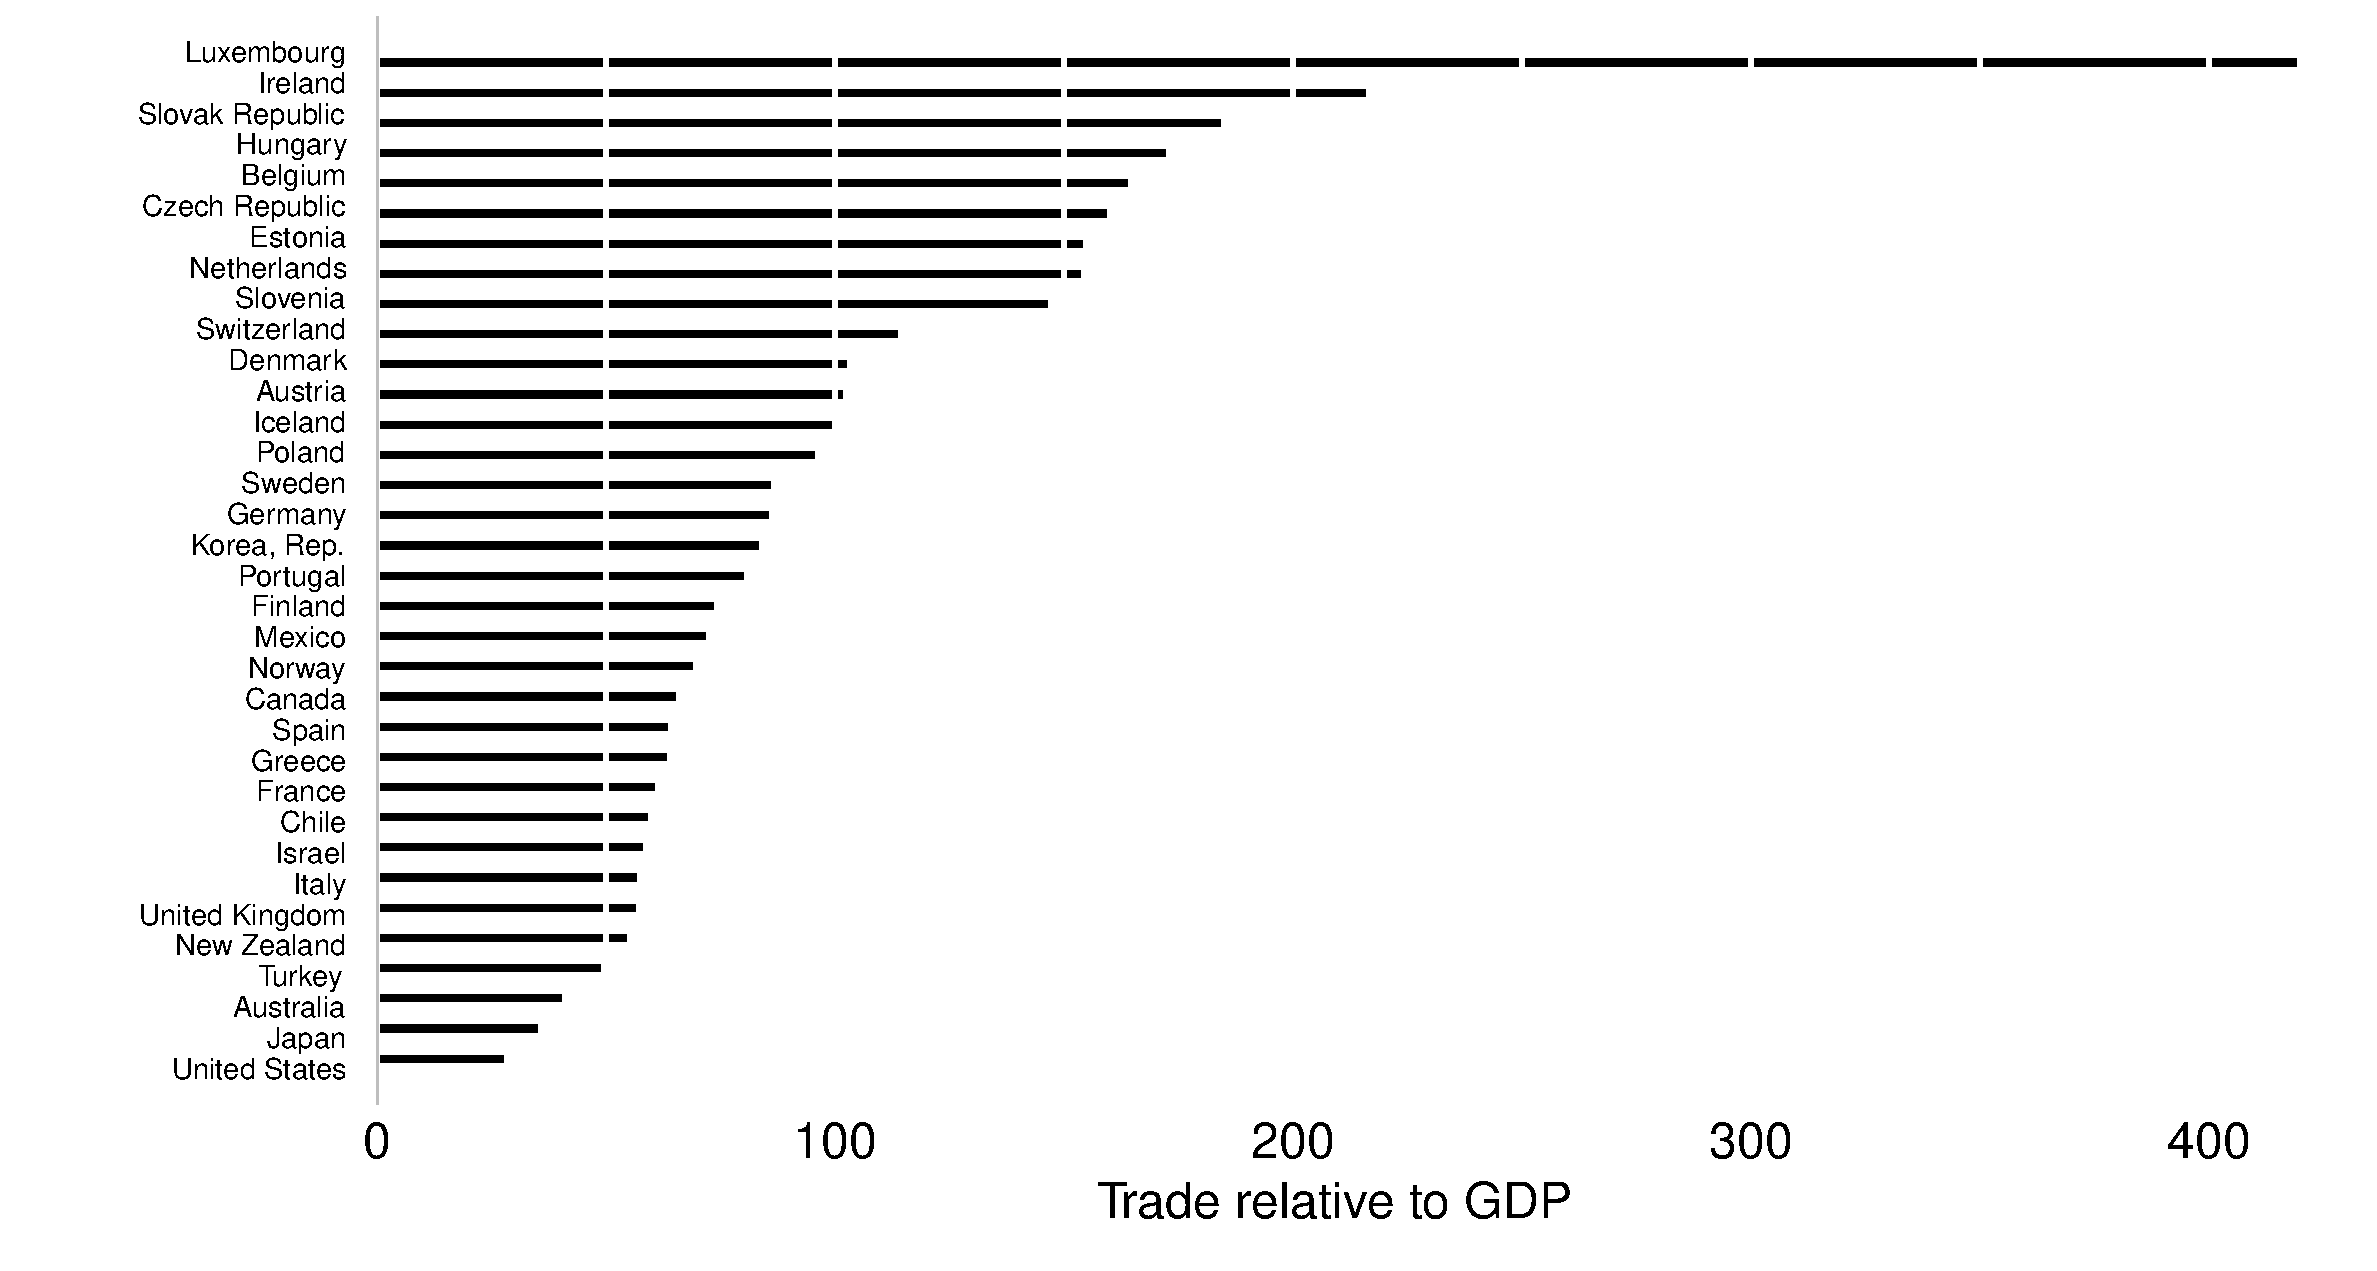
\includegraphics[scale=.3]{trade_to_gdp}
  \end{figure}  
\end{frame}
%--------------------------------------


%--------------------------------------
\begin{frame}
  Terms of trade (ToT) captures the relative price of exported versus imported goods
  \begin{align*}
    \frac{P_X}{P_M}*100
  \end{align*}
  The terms of trade increase when 
  \begin{enumerate}
    \item Export prices, $P_X$ increase
    \item Import prices, $P_M$ decrease
  \end{enumerate}
  \medskip
  An increase in the ToT increases general welfare  
    \begin{itemize}
      \item For every unit of export sold it can buy buy more units of imported goods
    \end{itemize}
\end{frame}
%--------------------------------------

%--------------------------------------
\begin{frame}{}
  \begin{figure}
    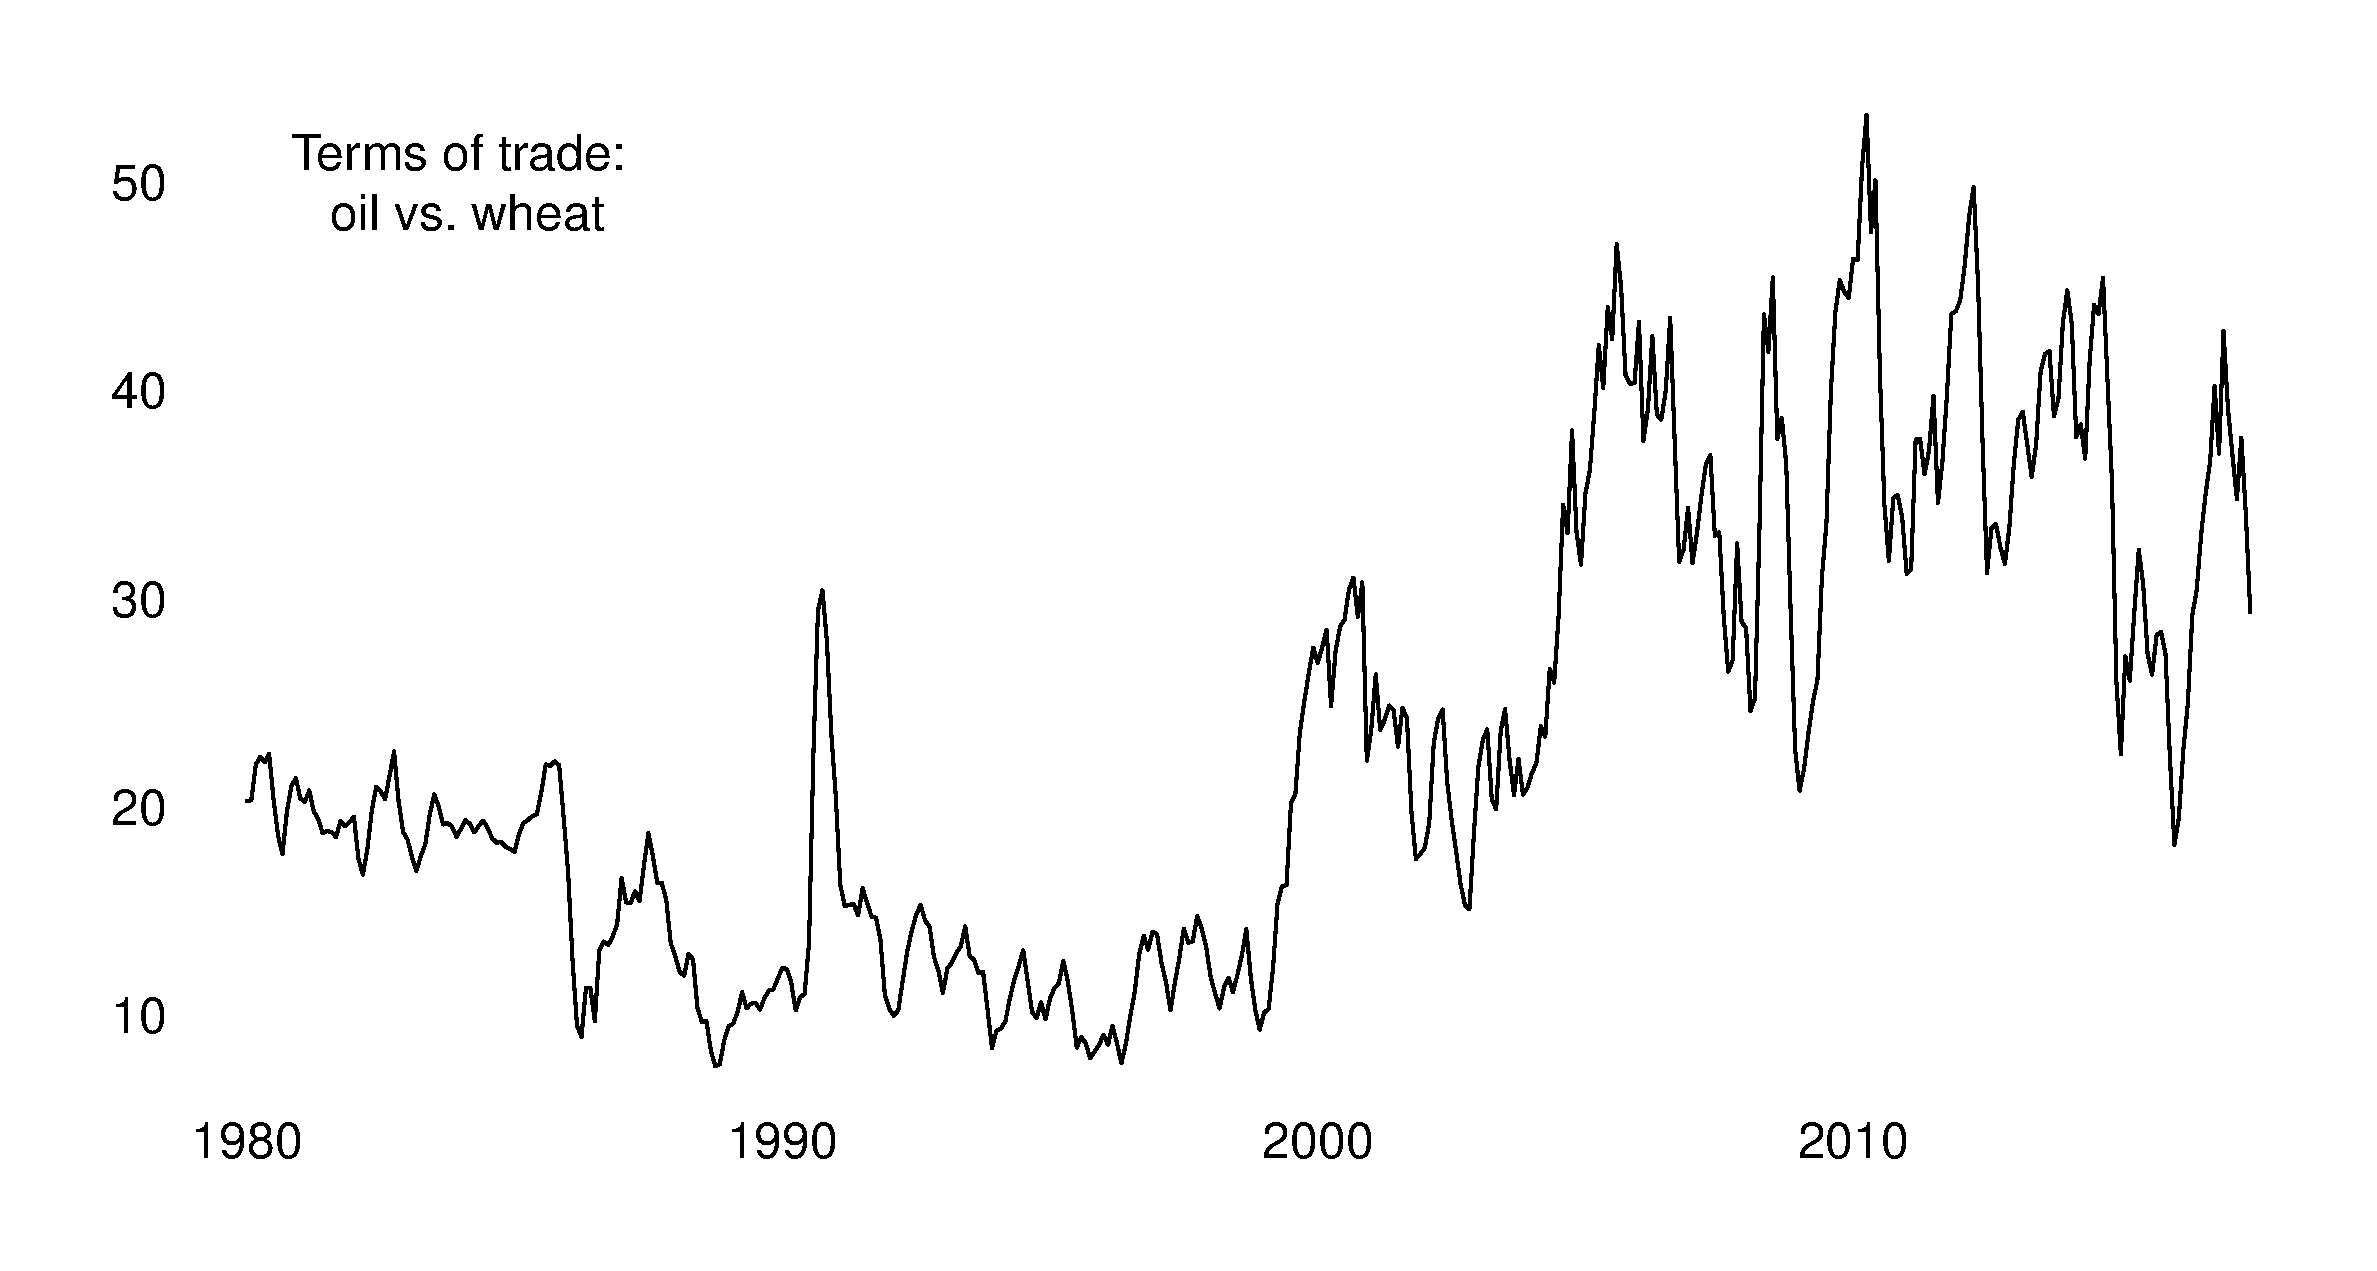
\includegraphics[scale=.3]{tot_example}
  \end{figure}  
\end{frame}
%--------------------------------------

%--------------------------------------
\begin{frame}{Terms of trade Australia}
  \begin{figure}
    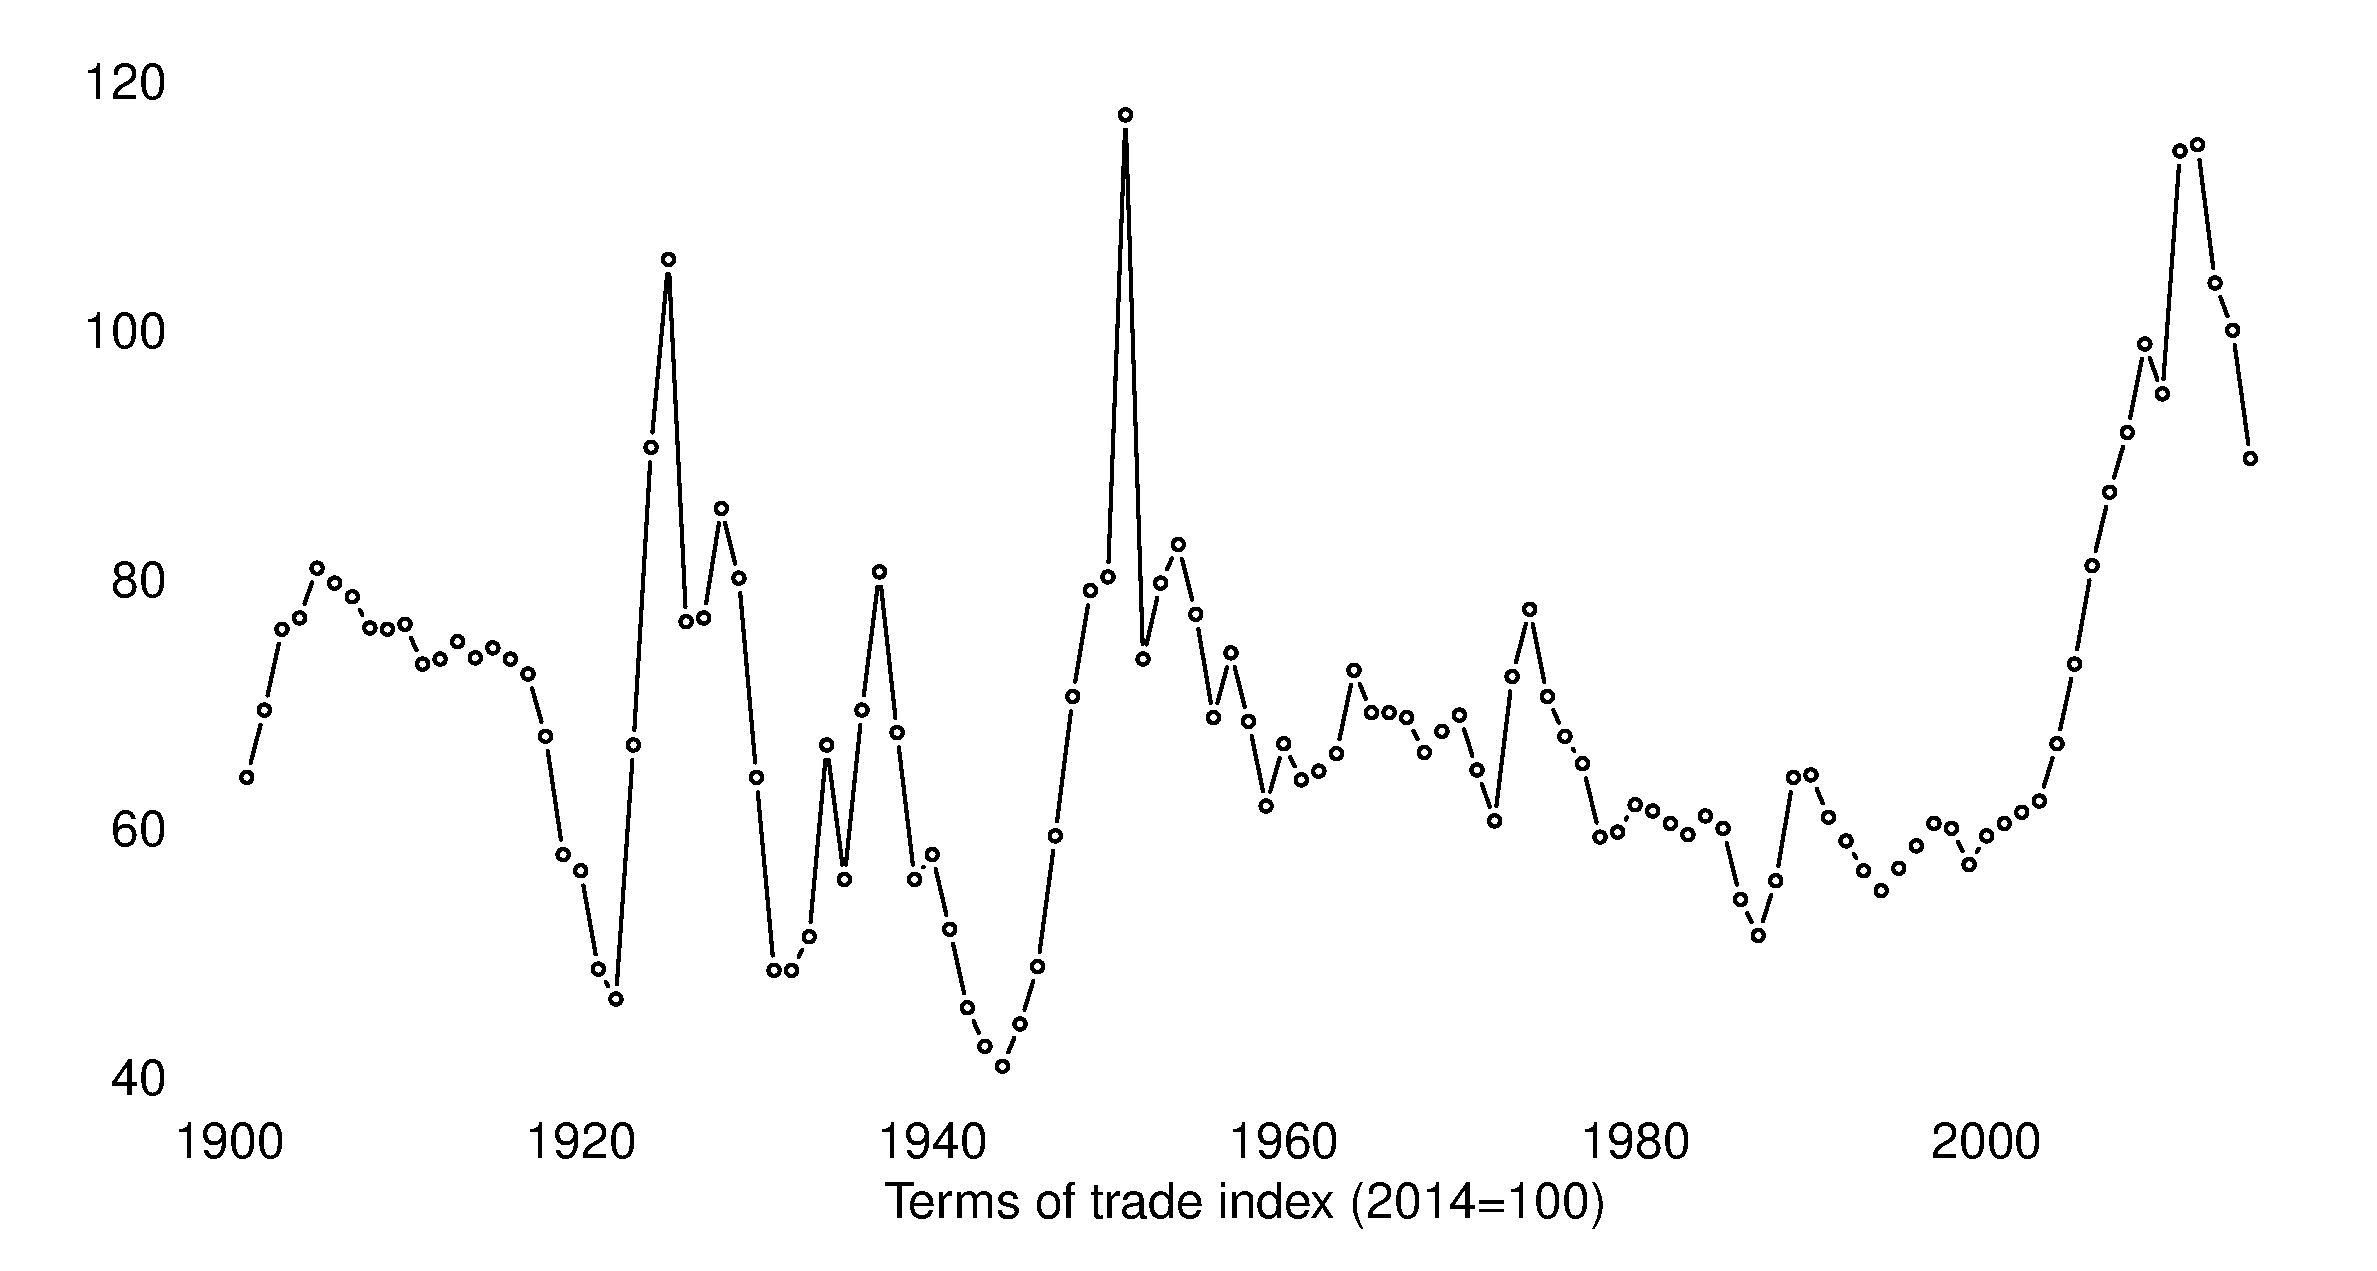
\includegraphics[scale=.3]{australia_tot}
  \end{figure}  
\end{frame}
%--------------------------------------


%--------------------------------------
\begin{frame}
  \begin{figure}
    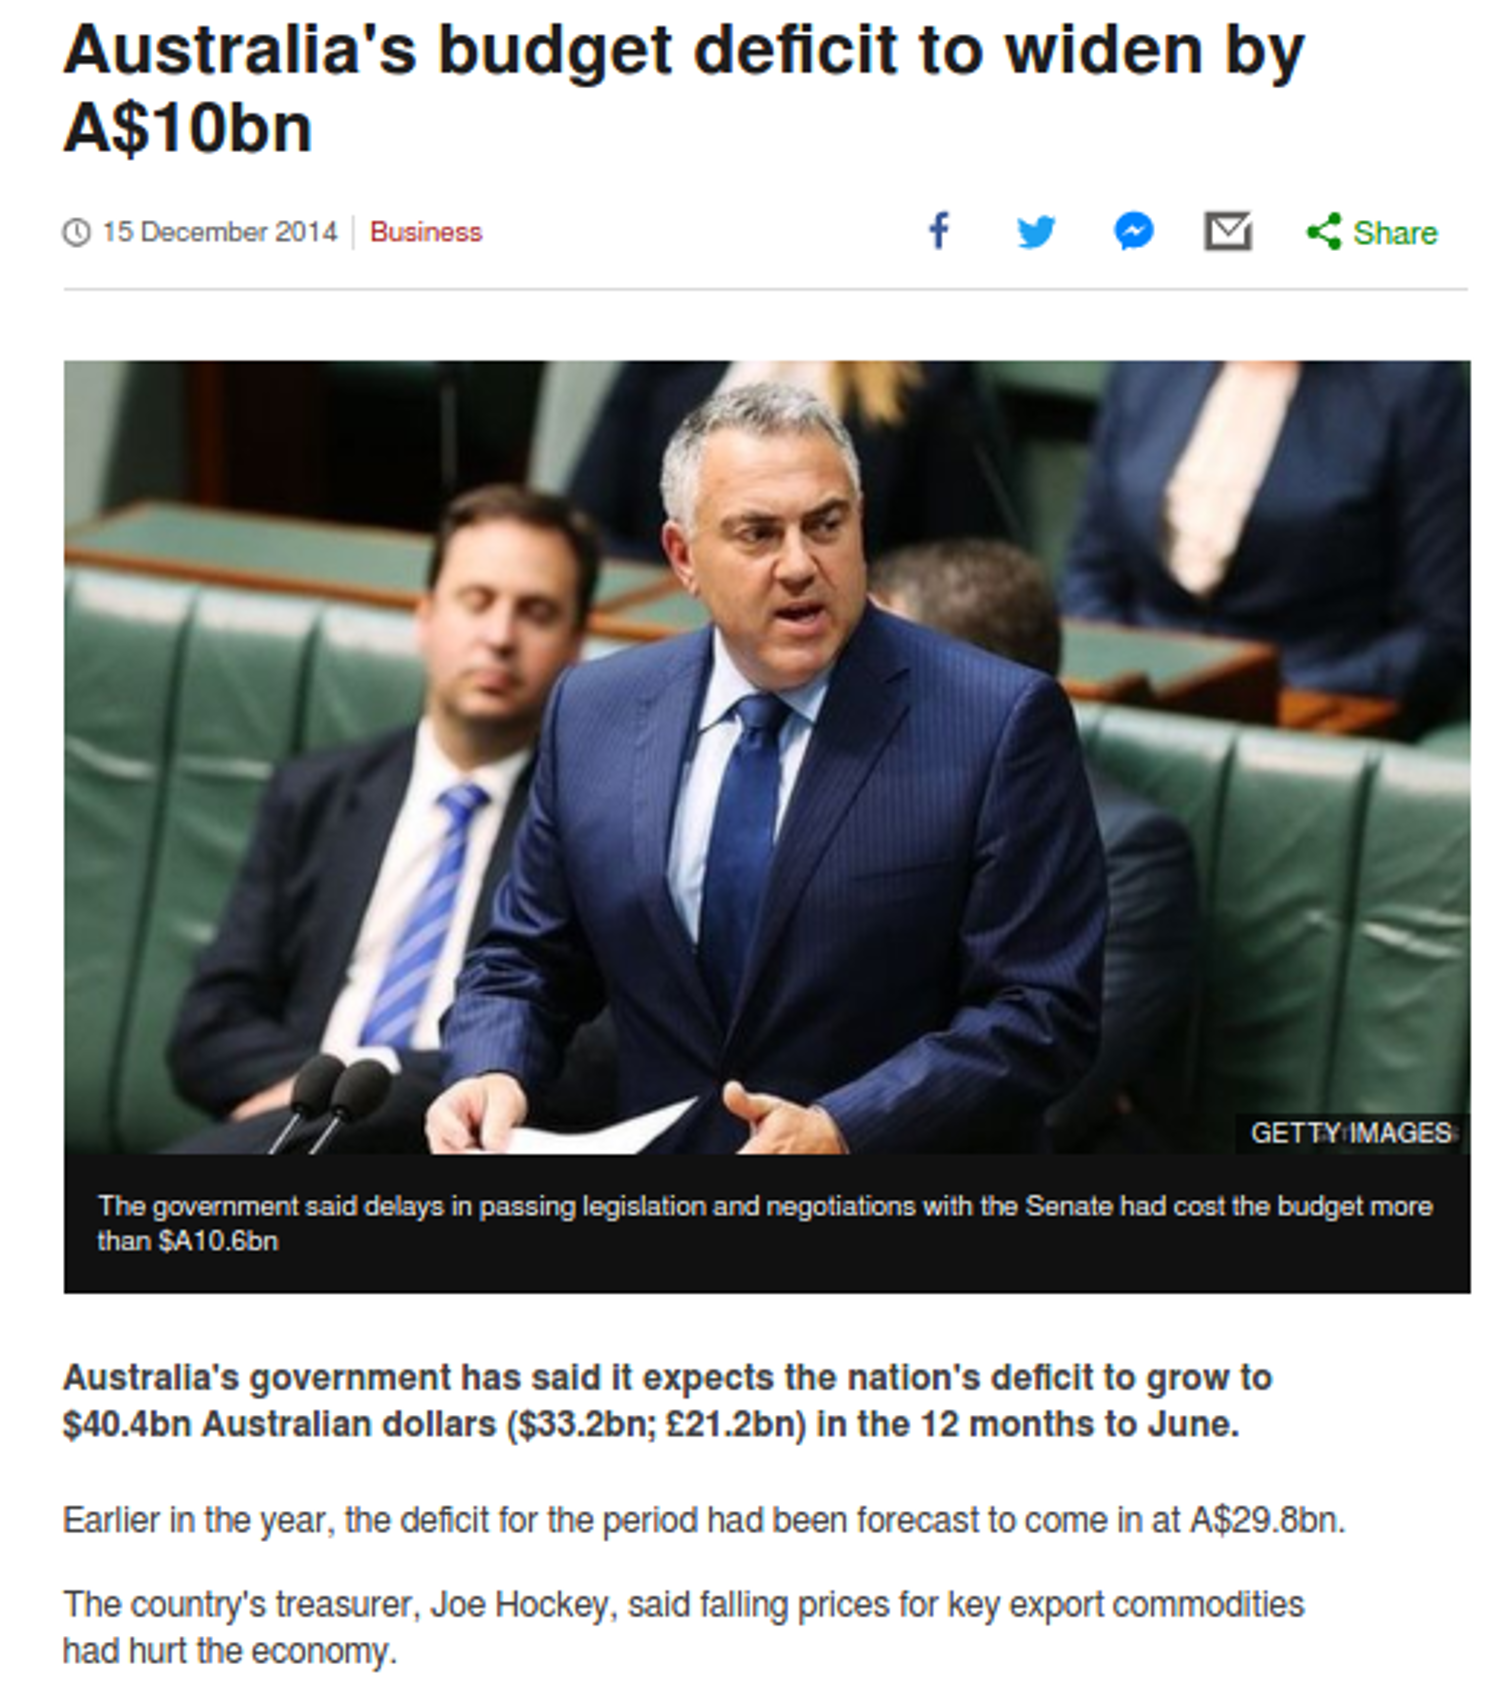
\includegraphics[scale=.7]{aus_budget}
  \end{figure}  
\end{frame}
%--------------------------------------

%--------------------------------------
\begin{frame}{UK imports and exports over time as ratio of GDP}
  \begin{figure}
    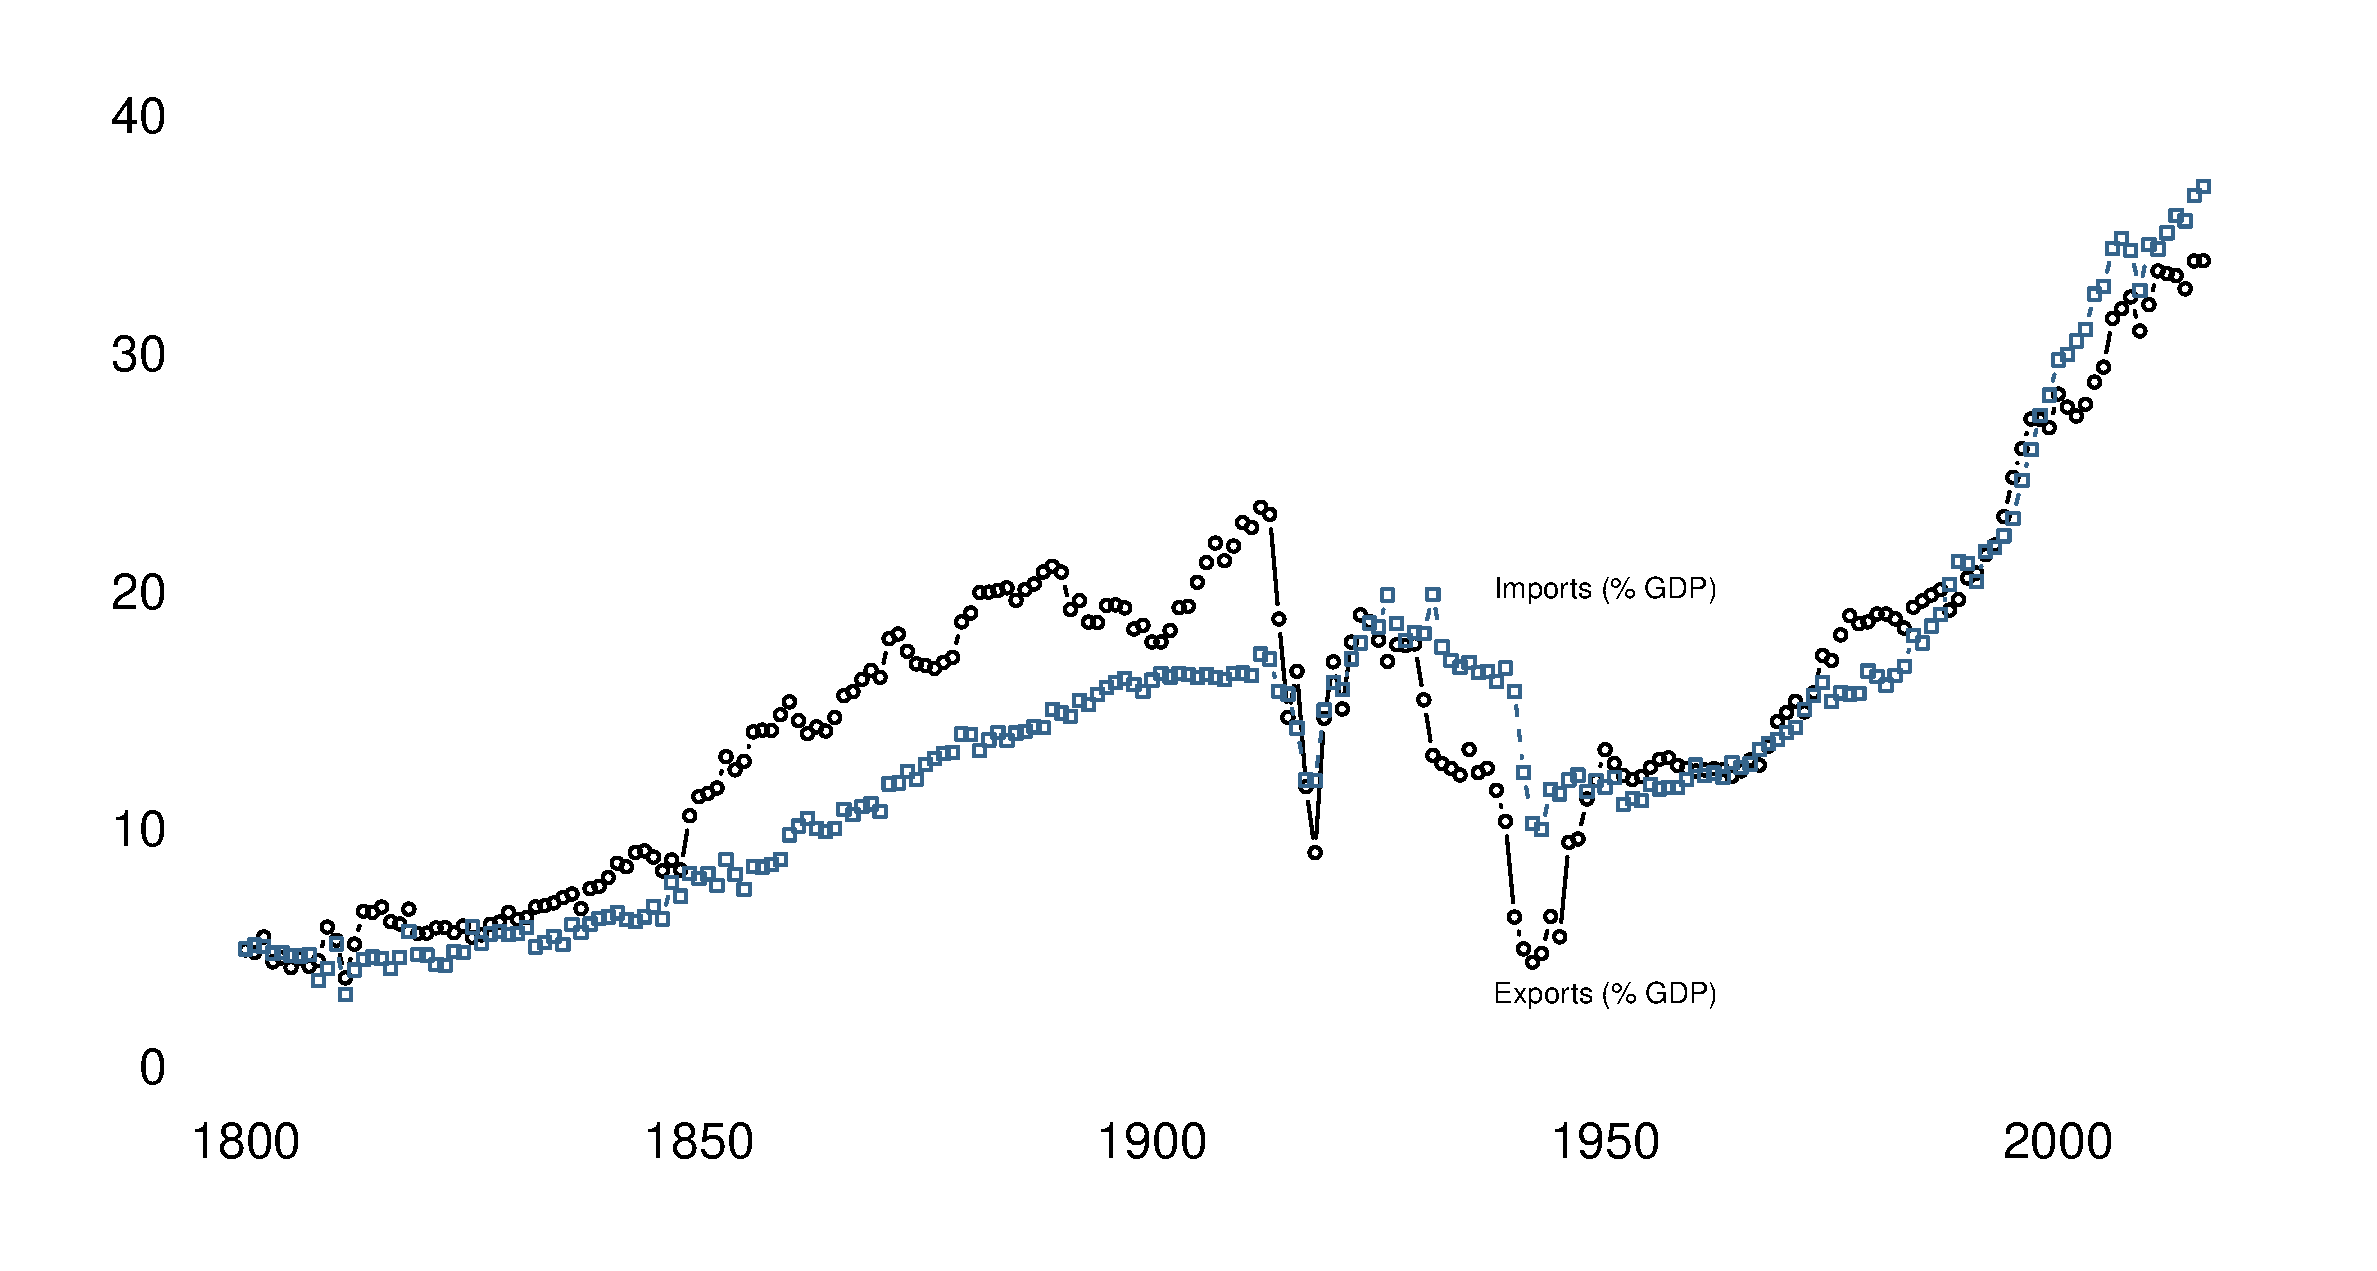
\includegraphics[scale=.3]{uk_trade}
  \end{figure}
  
\end{frame}
%--------------------------------------

%--------------------------------------
\begin{frame}{World trade shares per region for 2012}
  \begin{table}
    \begin{tabular}{lcc}
    Region      & Exports   & Imports\\
    \hline \\[-1.8ex]\\	
    Africa      & 3.5   & 3.3\\
    Asia        & 33.2  & 33.4\\
    Commonwealth of Independent States
                & 4.3   & 3.1\\
    Europe      & 34.7  & 35.1\\
    \hspace{3mm} EU internal trade  
                & 19.8  & 19.5\\
    Middle East & 7.3   & 3.9\\
    North America & 12.9  & 17.2\\
    South and Central America & 4.1 & 4.1\\      
    \end{tabular}
  \end{table}  
\end{frame}
%--------------------------------------

%--------------------------------------
\begin{frame}{}
 European trade flows are large
 \begin{itemize}
   \item Many countries, zero tariffs
 \end{itemize}
 \medskip
 Asian trade rivals that of Europe
 \begin{itemize}
   \item Cheap labour in China, Bangladesh, Vietnam, Cambodia
   \item Efficient production of high quality goods in Japan, South Korea
 \end{itemize}
 \medskip
 Former USSR and Middle East account for 10\% of world trade
 \begin{itemize}
   \item Exports of oil and natural gas
 \end{itemize}
 \medskip
 Low trade levels in South and Central America, but growing while Africa accounts for just 3.5\% of world trade
 \begin{itemize}
   \item Very marginal given population size
   \item Largely dependent on primary commodities
 \end{itemize}  
\end{frame}
%--------------------------------------

%--------------------------------------
\begin{frame}{Major shipping routes}
\framesubtitle{source: Nicolas Rapp}
  \begin{figure}
    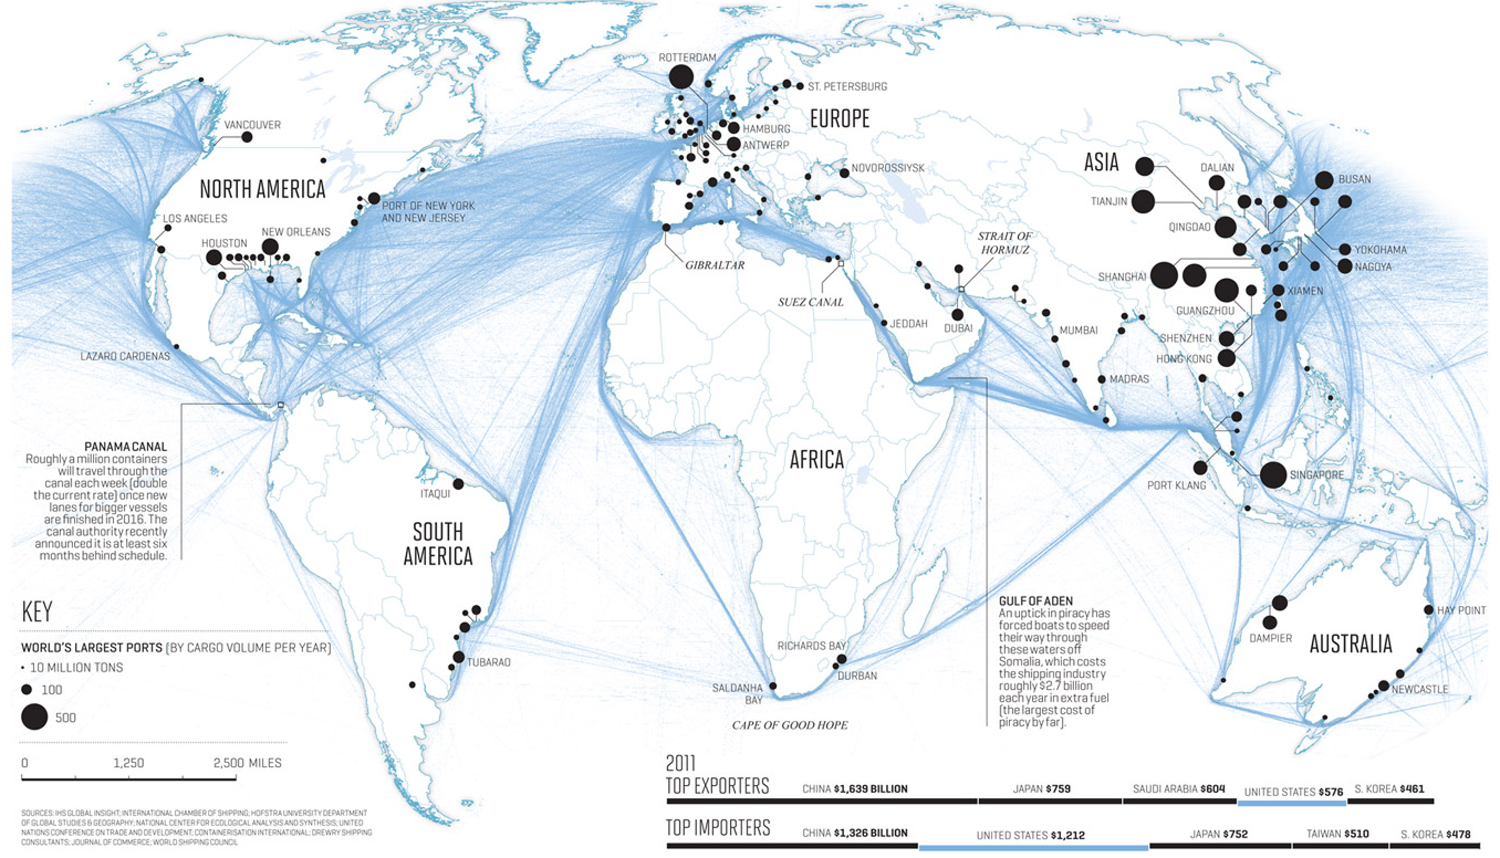
\includegraphics[scale=.8]{shipping}
  \end{figure}
\end{frame}
%--------------------------------------

%--------------------------------------
\begin{frame}{World merchandise trade flows Nov-Dec 2012}
\framesubtitle{source: Barclays research}
  \begin{figure}
    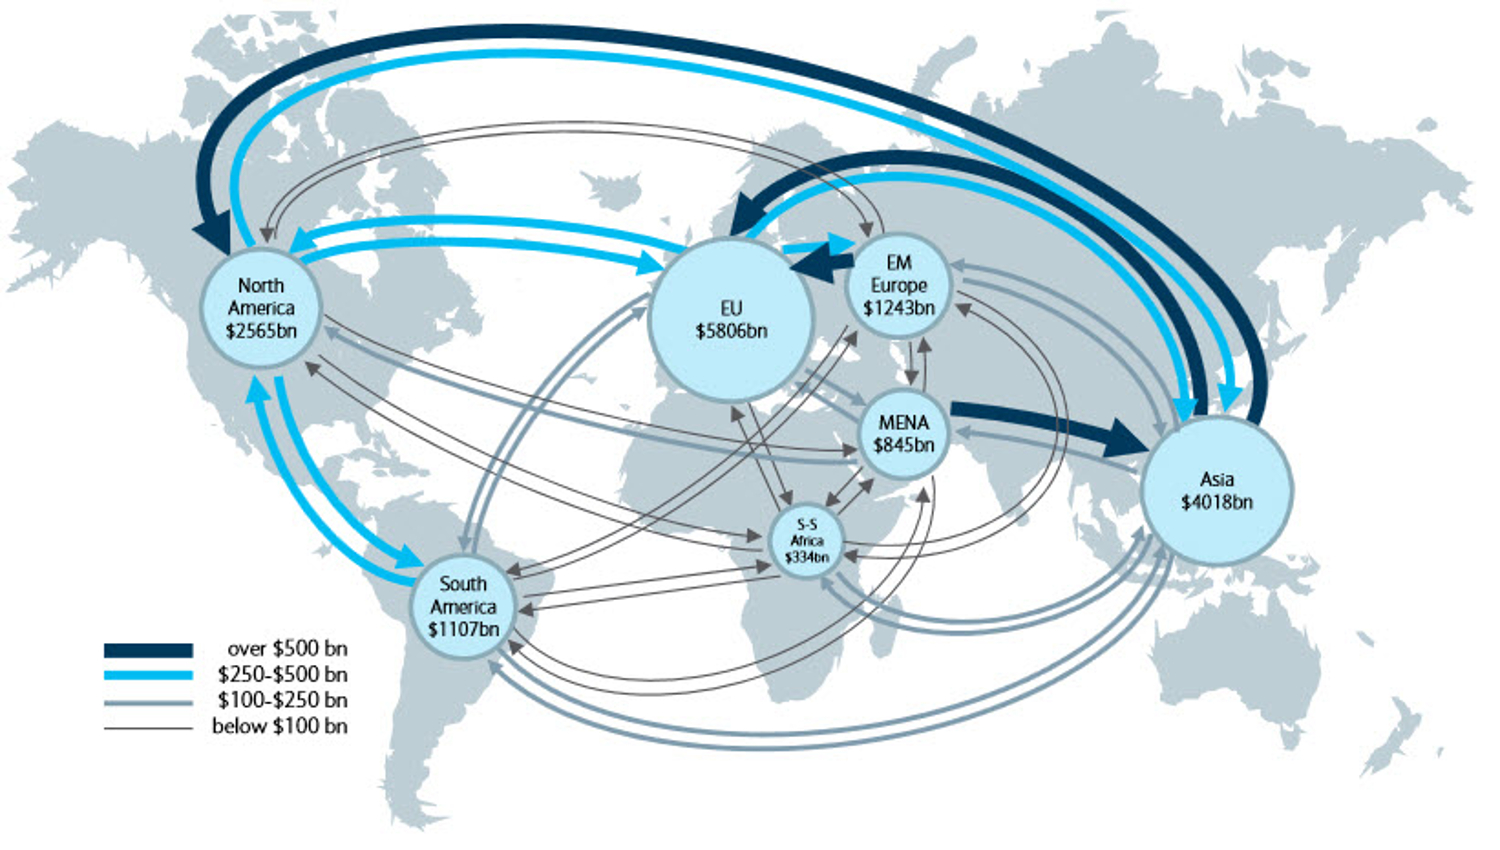
\includegraphics[scale=.2]{barclays}
  \end{figure}
\end{frame}
%--------------------------------------

%--------------------------------------
\begin{frame}
  There are large differences in trade across regions which are due to
    \begin{enumerate}
      \item Import tariffs
      \item Transportation costs
      \item Other factors such as conflict
    \end{enumerate}
    \medskip
  Trade barriers refer to all factor that influence the amount of goods/services shipped across international borders
  \begin{itemize}
    \item Trade barriers change over time as a result of changes in policies, technology, etc. 
  \end{itemize}
\end{frame}
%--------------------------------------

%--------------------------------------
\begin{frame}{UK export volumes}
  \begin{figure}
    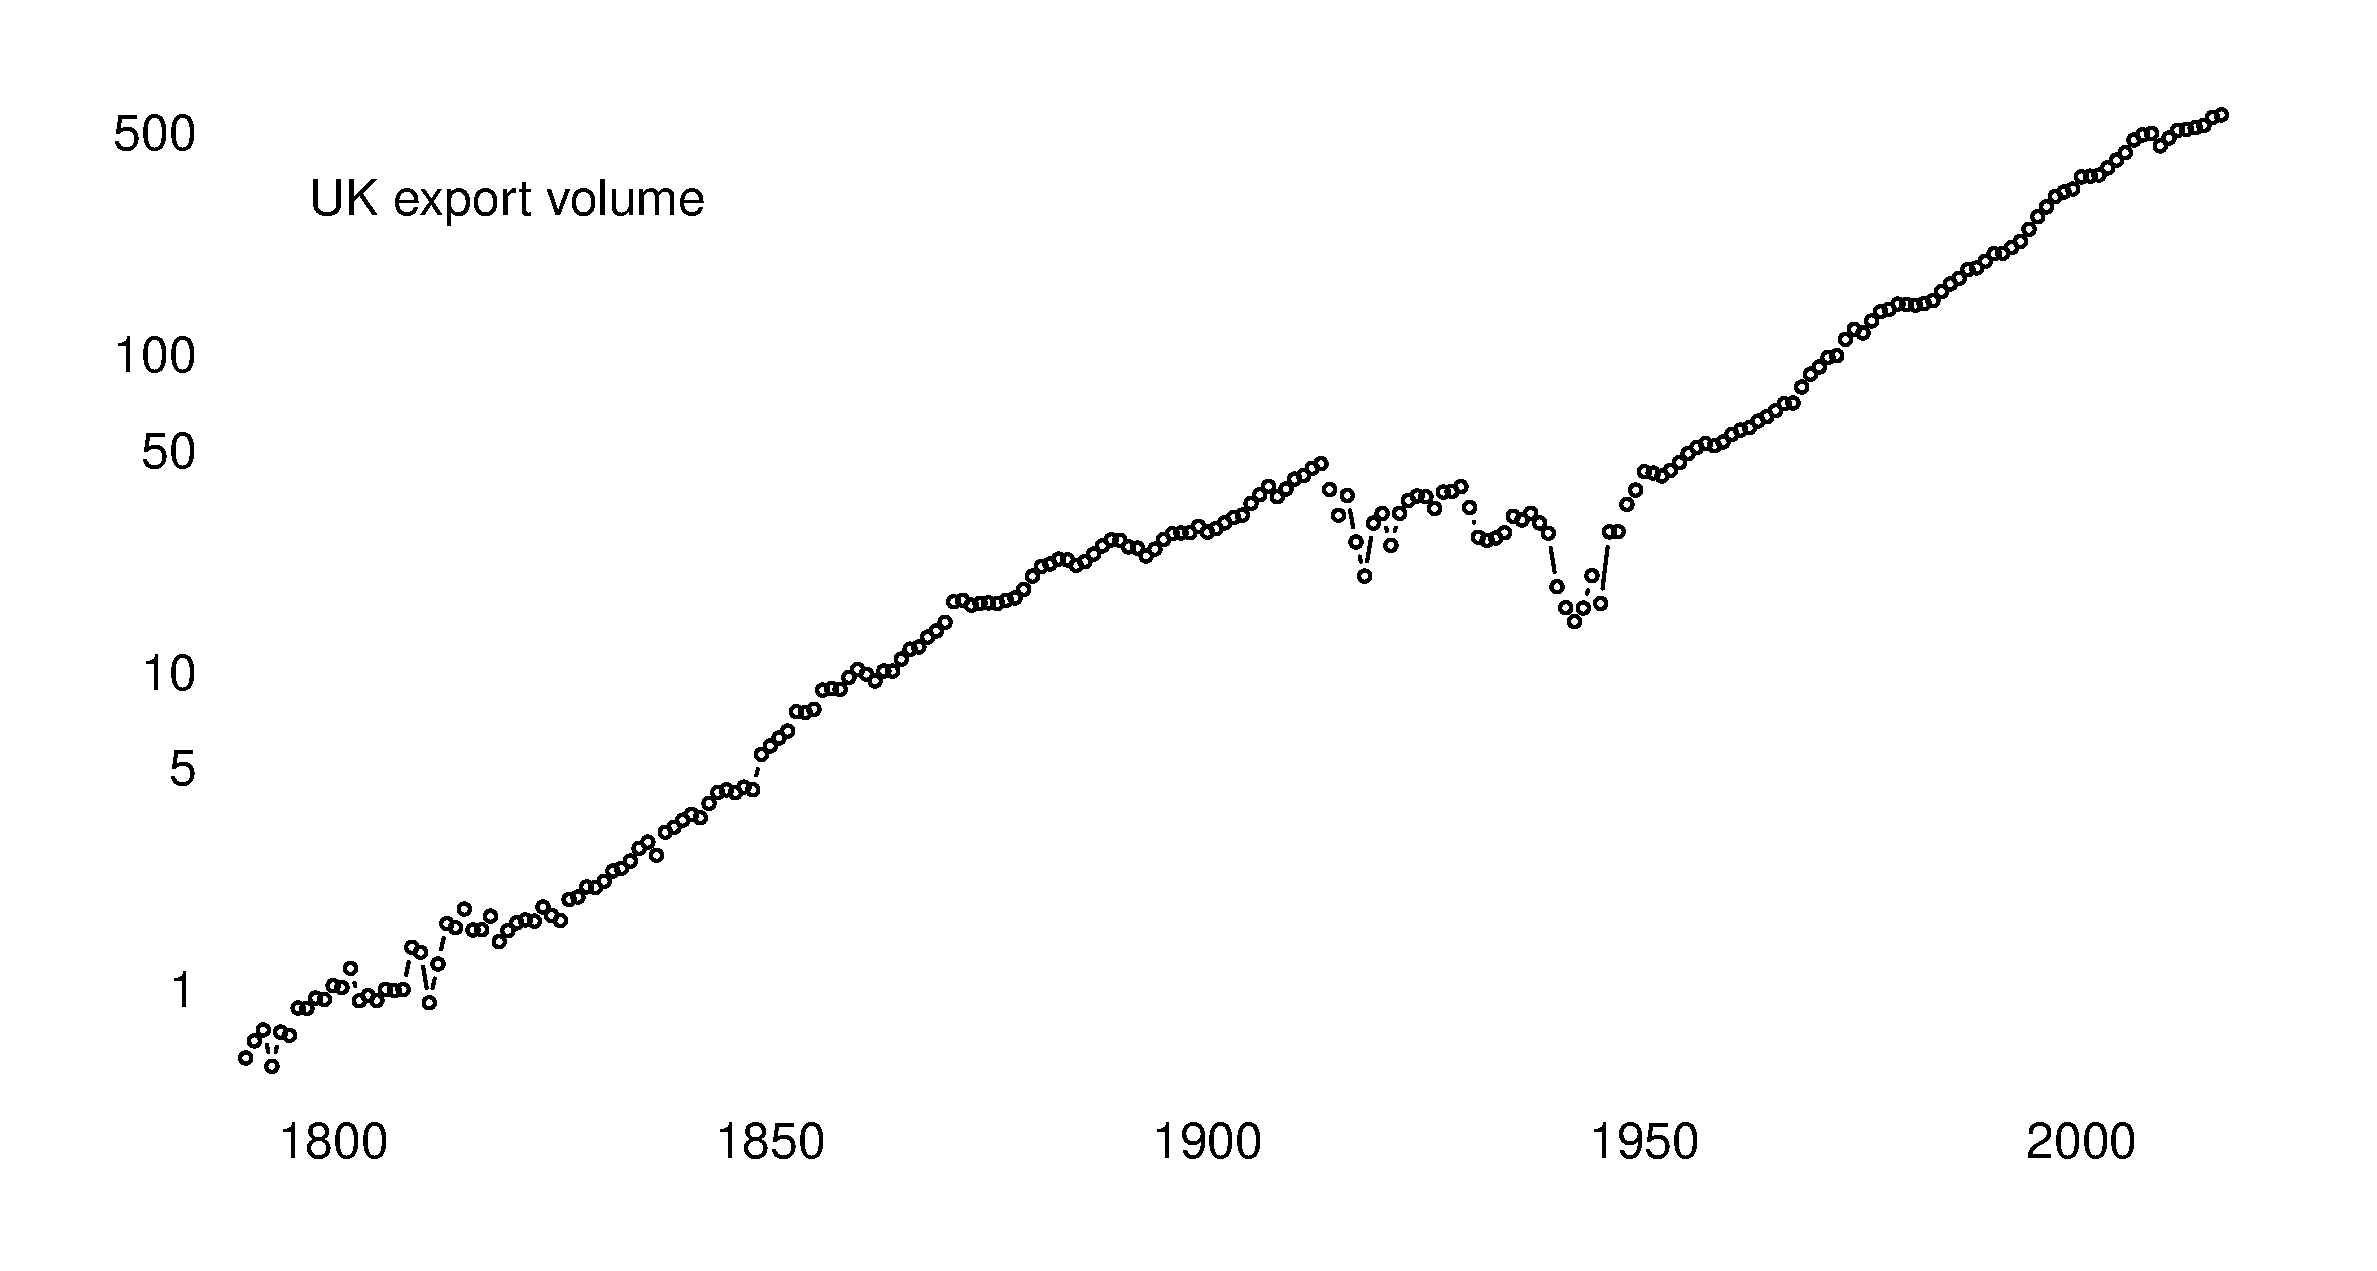
\includegraphics[scale=.3]{uk_exports}
  \end{figure}
  
\end{frame}
%--------------------------------------



%--------------------------------------
\begin{frame}{}
First golden age of trade between 1890-1913
\begin{itemize}
  \item Significant technological improvements, e.g. steamships, railroads, telephones, refrigeration
\end{itemize}
\medskip
This ended with the First World War which led to a large decrease in trade during the interbellum (1918-1939)
\begin{itemize}
  \item Trade decline due to Great Depression
  \item Increase in world-wide tariff rate of 25\%, trade decline of about 33\%
\end{itemize}
\medskip
Second golden age of trade since 1950s
\begin{itemize}
  \item Low tariffs through GATT, later WTO
  \item Improved transportation, e.g. shipping container (1956)
  \item Trade surpassed pre-WWI levels
\end{itemize}  
\end{frame}
%--------------------------------------

%--------------------------------------
\begin{frame}{Trade composition between 1900-1960}
  \begin{figure}
    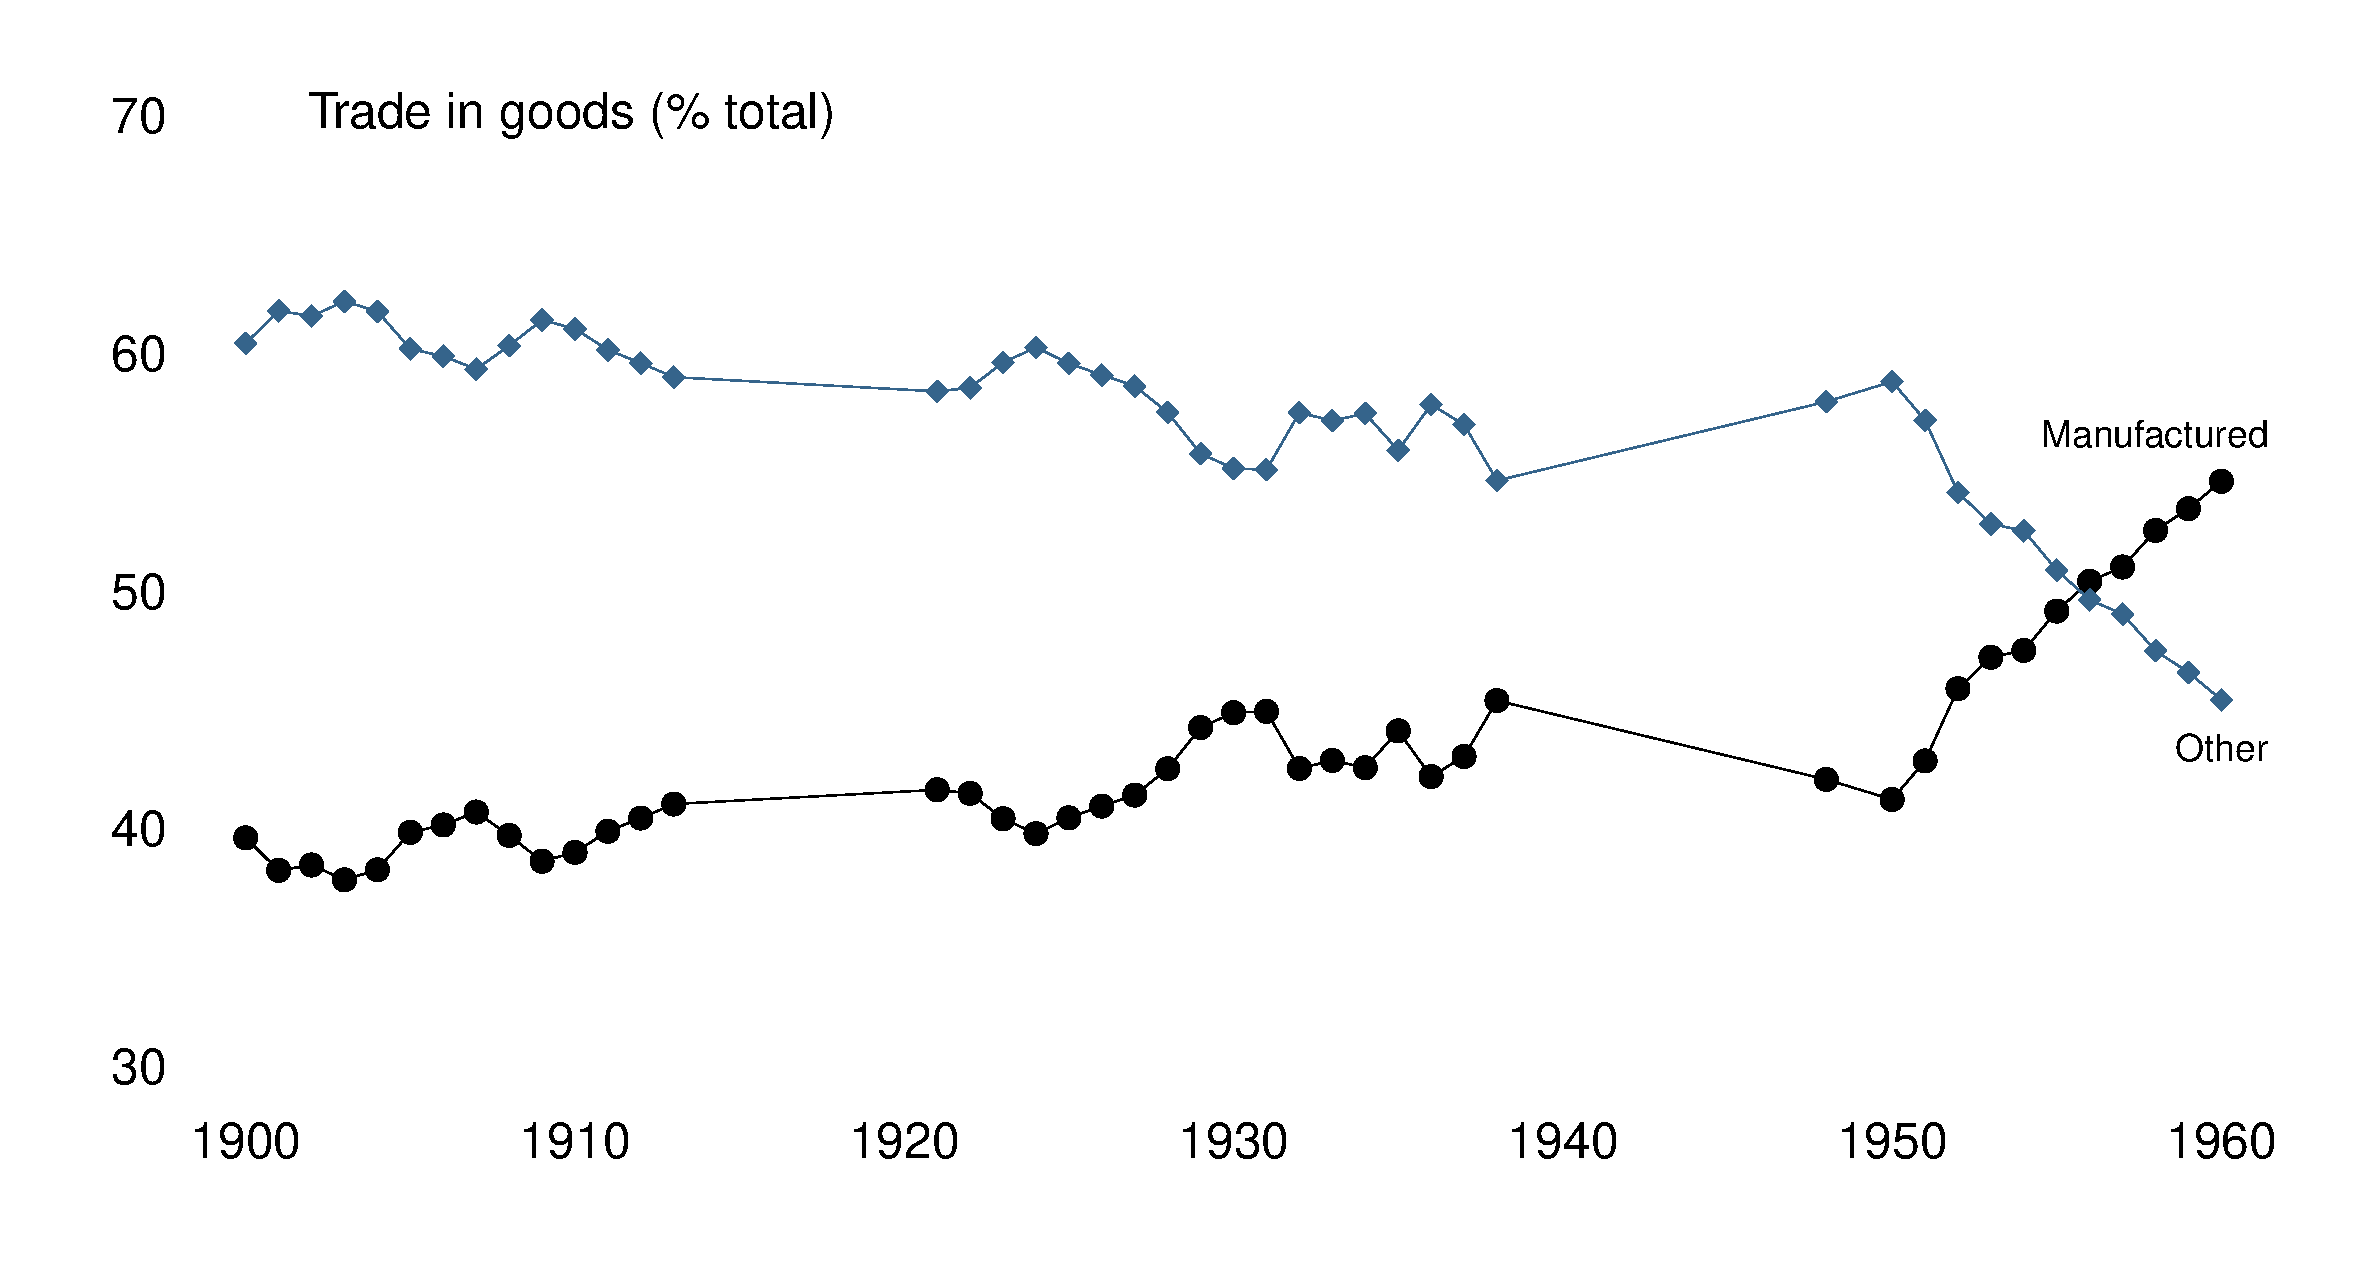
\includegraphics[scale=.3]{world_trade}  \end{figure}
  
\end{frame}
%--------------------------------------

%--------------------------------------
\begin{frame}{}
Current trade composition is roughly
\medskip
\begin{itemize}
  \item 50\% manufactured goods
  \begin{itemize}
    \item clothing from low-wage countries, capital-intensive goods from industrialised countries
  \end{itemize}
  \medskip
  \item 20\% services (e.g. transport, tourism, insurance)
  \medskip
  \item 20\% mining products
  \begin{itemize}
    \item Fossil fuels from America, Australia, and the Middle East
    \item Natural resources such as copper from Chile and those conflict minerals from Congo for your telephone
  \end{itemize}
  \medskip
  \item 10\% agricultural products
  \begin{itemize}
    \item e.g. food from the EU and Latin America, cotton from India, timber from West Africa
  \end{itemize}
\end{itemize}  
\end{frame}
%--------------------------------------

%--------------------------------------
\begin{frame}
  \begin{figure}\centering
    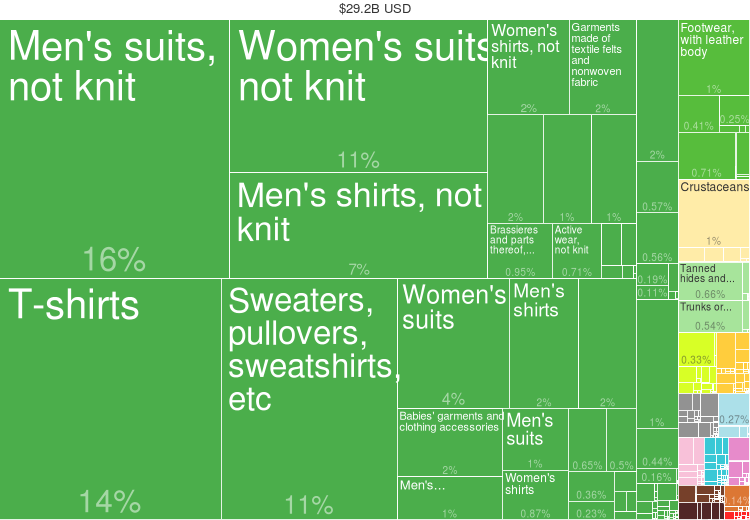
\includegraphics[scale=.4]{bangladesh}
  \end{figure}
\end{frame}
%--------------------------------------

%--------------------------------------
\begin{frame}
  \begin{figure}\centering
    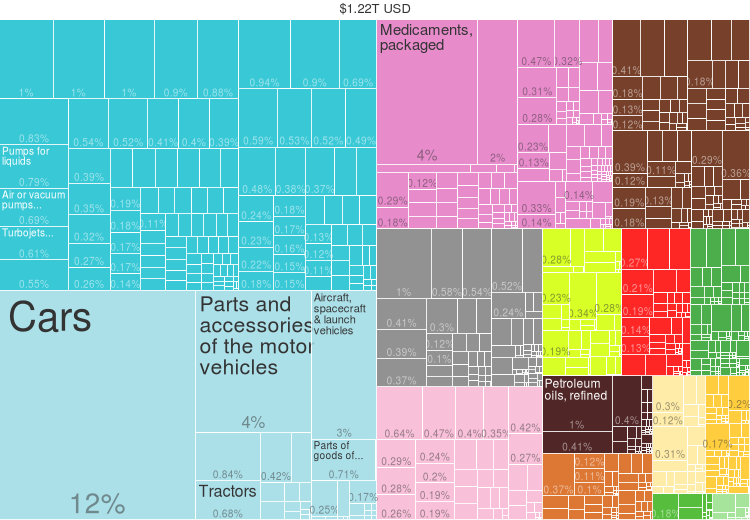
\includegraphics[scale=.4]{germany}
  \end{figure}
\end{frame}
%--------------------------------------

%--------------------------------------
\begin{frame}
  \begin{figure}\centering
    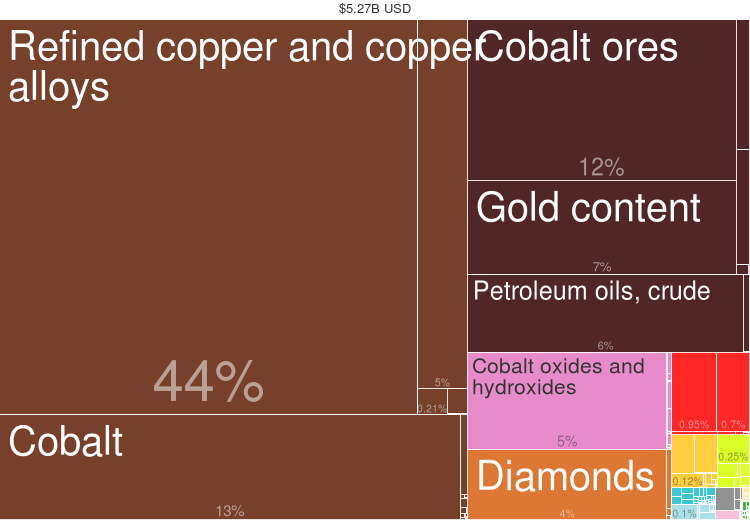
\includegraphics[scale=.4]{congo_dr}
  \end{figure}
\end{frame}
%--------------------------------------

%--------------------------------------
\begin{frame}
  \begin{figure}\centering
    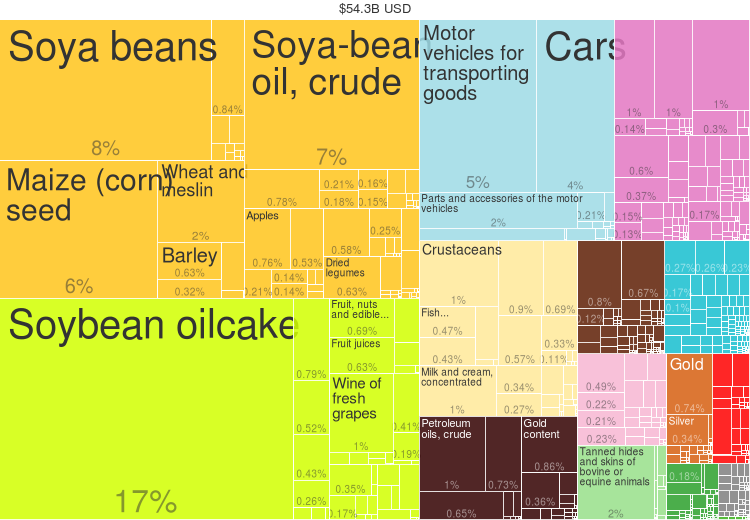
\includegraphics[scale=.4]{argentina}
  \end{figure}
\end{frame}
%--------------------------------------

%--------------------------------------
\begin{frame}
  \begin{figure}\centering
    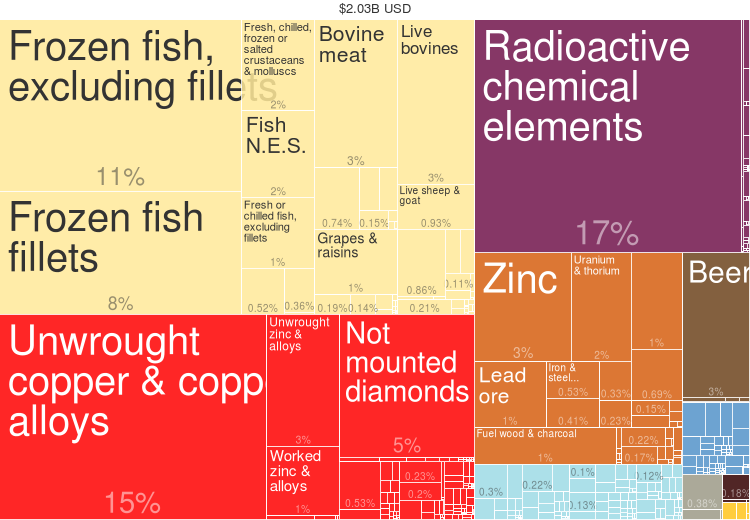
\includegraphics[scale=.4]{namibia}
  \end{figure}
\end{frame}
%--------------------------------------

%--------------------------------------
\begin{frame}{}
Differences in geographic factors such as climate and natural resources explains why Congo DR exports metals and Argentina soybeans.
\newline
The fact that Bangladesh exports clothing and Germany cars stems from difference in
\begin{itemize}
  \item Labour productivity
  \item Relative supply of production factors such as capital and labour, and their used in production of different goods
\end{itemize}
  \bigskip
 \textbf{Food for thought:} Mexico is the world's largest exporter of fresh tomatoes; which country is the second largest?
\end{frame}
%--------------------------------------

%--------------------------------------
\begin{frame}{Foreign direct investments flows in 2015}
  \begin{figure}
    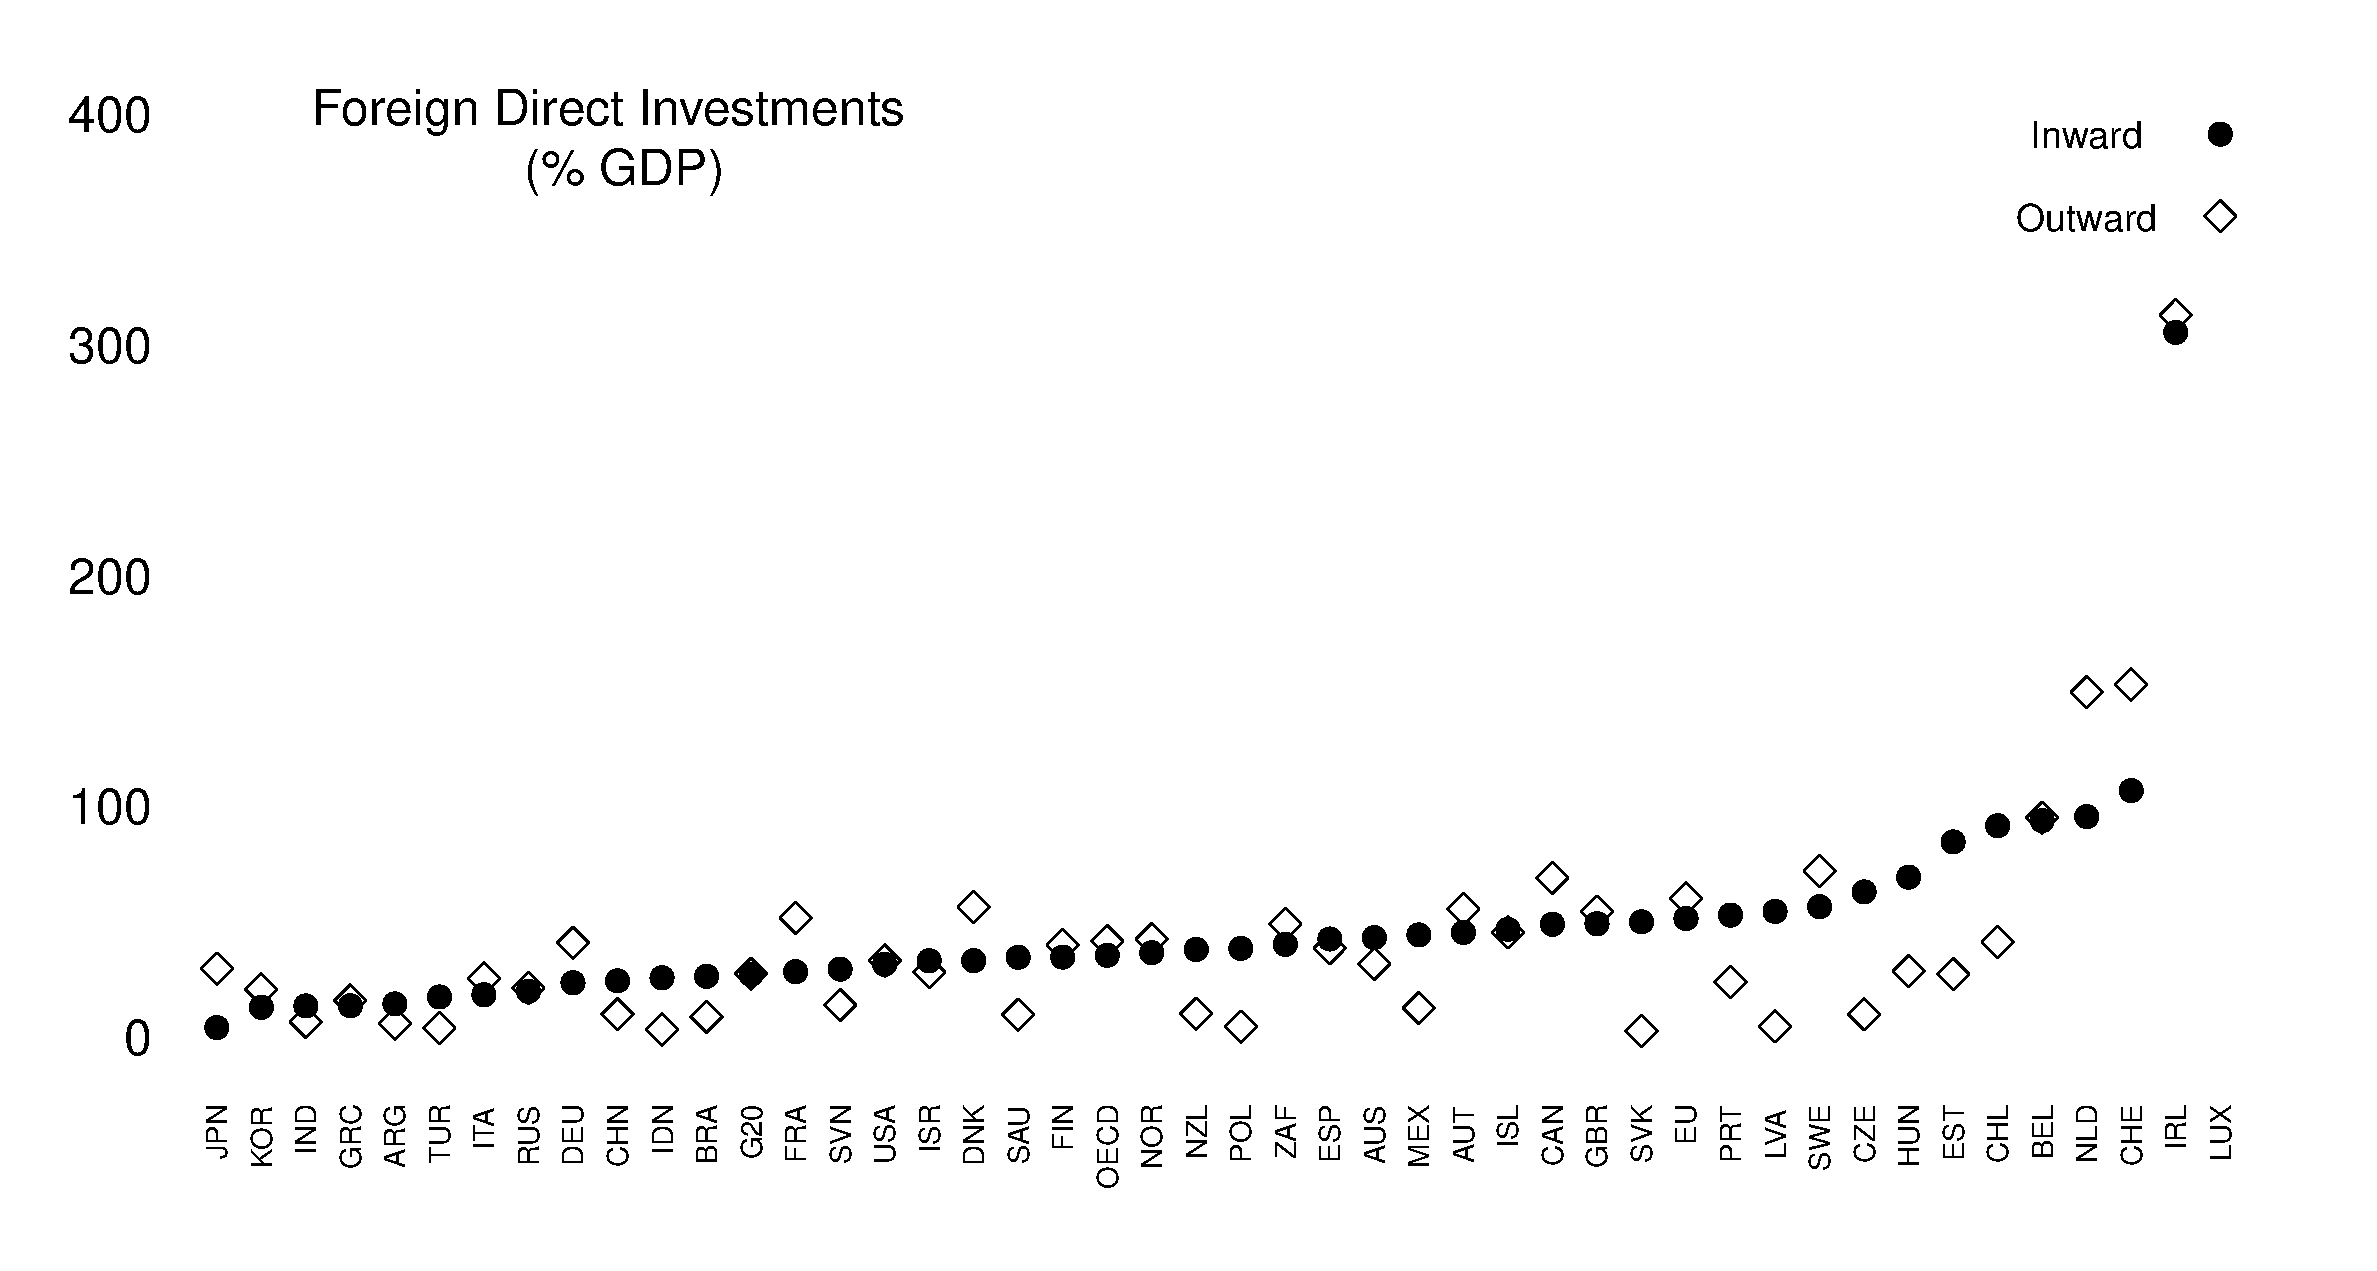
\includegraphics[scale=.3]{fdi}  
  \end{figure}  
\end{frame}
%--------------------------------------

%--------------------------------------
\begin{frame}{}
There are two types of FDI:
\medskip
\begin{enumerate}
  \item Horizontal: Firm from country $i$ owns company in country $j$ that has same production activity as domestic
  \begin{itemize}
    \item Allows firms to circumvent tariffs or quotas
    \item Better access to local market
    \item Sharing of technical expertise
  \end{itemize}
  \medskip
  \item Vertical: Firm from country $i$ owns company on country $j$ that operates a different stage of the production process
  \begin{itemize}
    \item Predominantly firms from industrialised countries owning factories in low-wage countries
    \item Reduces production costs
  \end{itemize}
\end{enumerate}  
\end{frame}
%--------------------------------------

%--------------------------------------
\begin{frame}{Migration flows between 2005-2010}
  \begin{figure}
    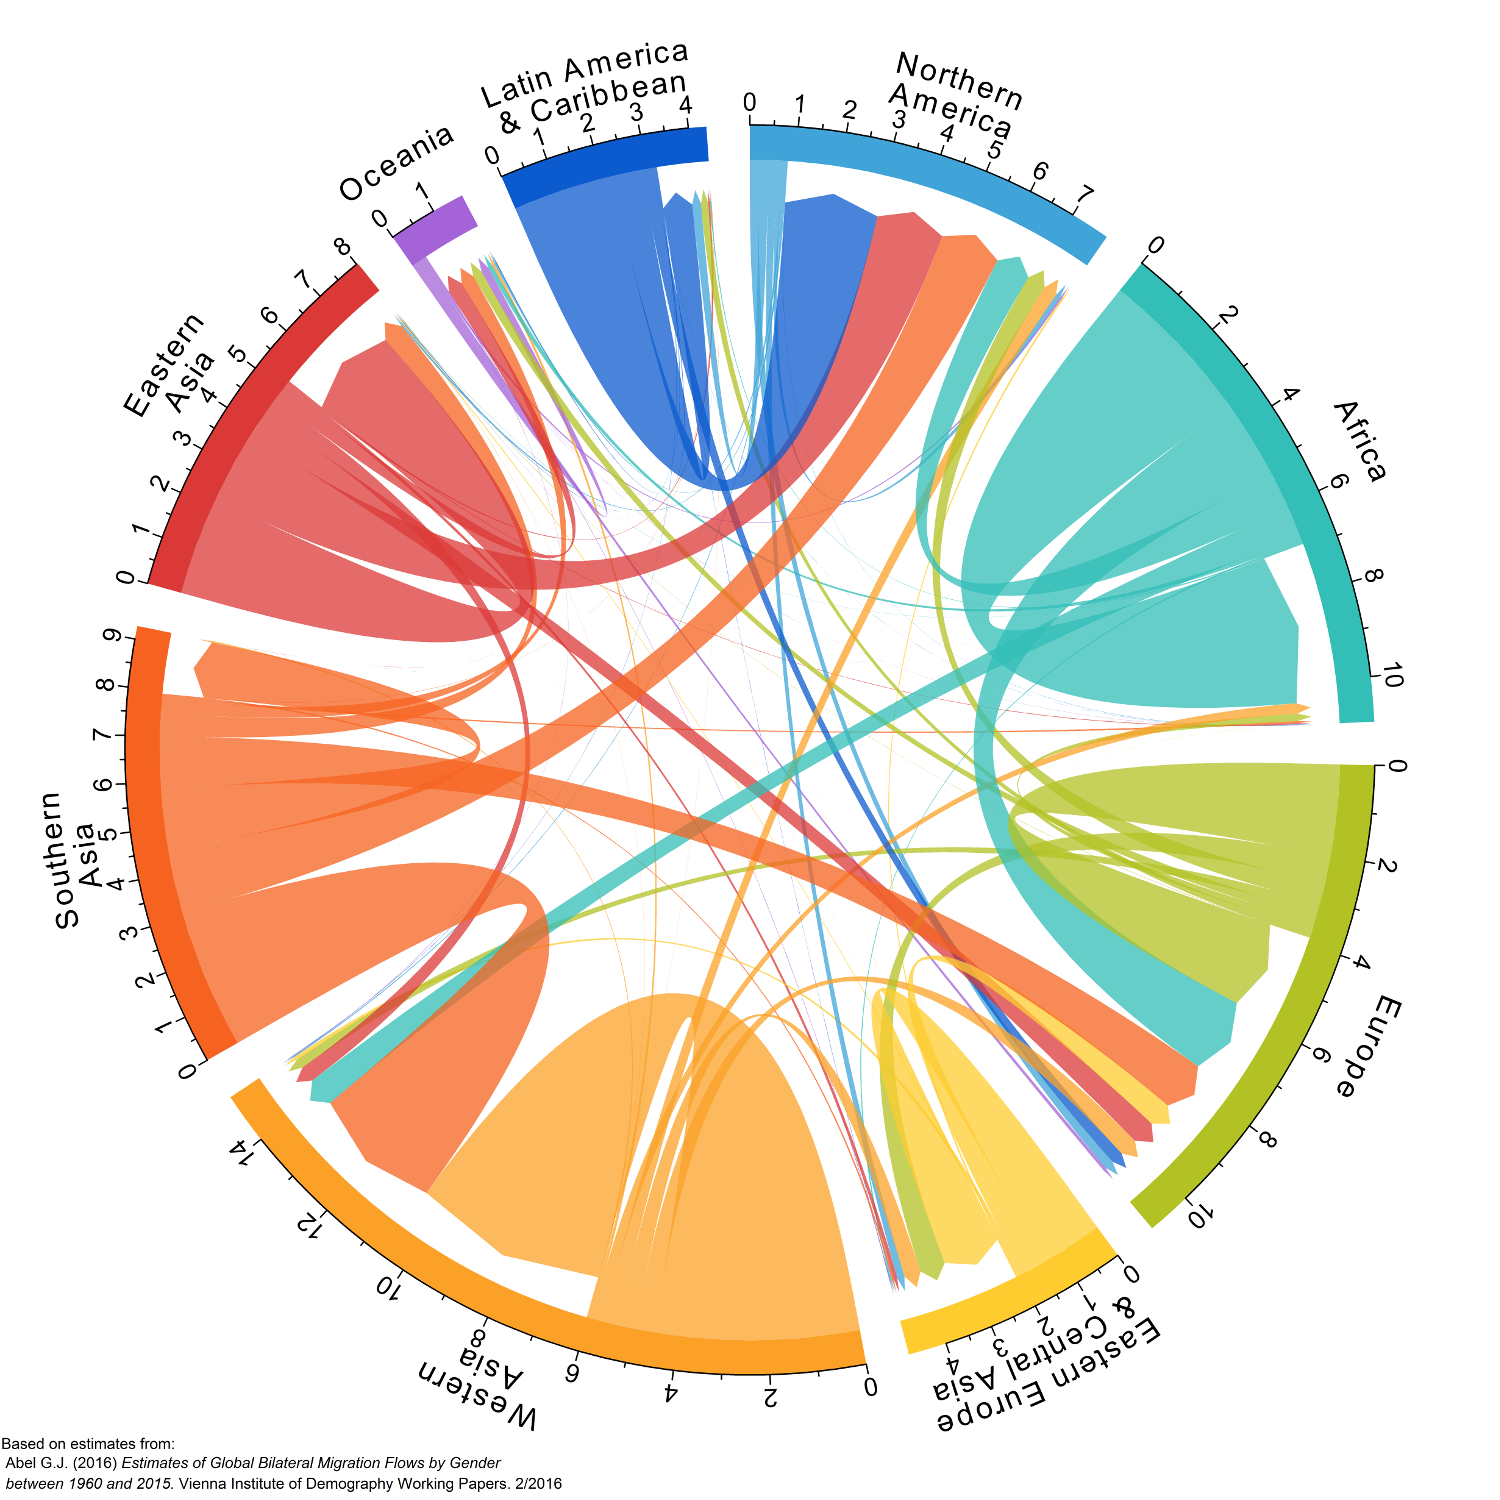
\includegraphics[scale=2]{migration}
  \end{figure}  
\end{frame}
%--------------------------------------

%--------------------------------------
\begin{frame}{}
  In contrast with FDI flows, most migration occurs in the developing world where migrants move to seek employment or other reasons such as conflict or famine.
  \begin{itemize}
    \item Migration is often stricter regulated that the flow of goods or capital
  \end{itemize}
  \bigskip
  From an economic perspective international trade can theoretically help reduce migrant flows
  \begin{enumerate}
    \item Trade can increase living standards in same way moving to a higher-wage country can
    \item More trade entails more workers needed in export industries
  \end{enumerate}
\end{frame}
%--------------------------------------


%--------------------------------------
\end{document}
